\documentclass[ALICE,manyauthors]{cernphprep}

%%%%%%%%%%%%% Define various directories %%%%%%%%%%%%%%%%%%%%%%%%%%%%%%
\newcommand{\ResultsDirBase}{/home/jesse/Analysis/FemtoAnalysis/Results/}
\newcommand{\ResultsDirBaseLamKch}{/home/jesse/Analysis/FemtoAnalysis/Results/Results_cLamcKch_20180505/}
\newcommand{\ResultsDirBaseLamKs}{/home/jesse/Analysis/FemtoAnalysis/Results/Results_cLamK0_20180505/}
\newcommand{\VZeroEffDirBase}{/home/jesse/Analysis/FemtoAnalysis/Results/V0Efficiency/}

\newcommand{\MomRes}{_MomResCrctn}%{}

\newcommand{\NonFlatBgdLamKch}{_NonFlatBgdCrctnLamK0LinearLamKchPolynomial}
\newcommand{\NonFlatBgdLamKs}{_NonFlatBgdCrctnLamK0LinearLamKchPolynomial}

\newcommand{\ResNum}{_3Res}
\newcommand{\PrimMaxDecay}{_PrimMaxDecay10fm}
\newcommand{\ResMethod}{_UsingXiDataAndCoulombOnly}

\newcommand{\ParamFixAndShareLamKch}{_ShareLam_Dualie_ShareLam_ShareRadii}
\newcommand{\ParamFixAndShareLamKs}{_ShareLam_Dualie_ShareLam_ShareRadii}

\newcommand{\SaveNameModLamKch}{\MomRes\NonFlatBgdLamKch\ResNum\PrimMaxDecay\ResMethod\ParamFixAndShareLamKch}
\newcommand{\SaveNameModLamKs}{\MomRes\NonFlatBgdLamKs\ResNum\PrimMaxDecay\ResMethod\ParamFixAndShareLamKs}


%%%%%%%% Shorthand definitions %%%%%%%%%%%%%%%%%%%%%%%%%%%%%%%%%%%%%%%%%%%%%%%%%%%%%%%%%%%%%
\newcommand{\kstar}{$k^{*}$\xspace}
\newcommand{\ktrue}{$k^{*}_{\mathrm{True}}$\xspace}
\newcommand{\krec}{$k^{*}_{\mathrm{Rec}}$\xspace}
\newcommand{\minv}{$m_{\mathrm{inv}}$\xspace}
\newcommand{\mt}{$m_{\mathrm{T}}$\xspace}
\newcommand{\pt}{$p_{\mathrm{T}}$\xspace}

\newcommand{\Lam}{$\Lambda$\xspace}
\newcommand{\ALam}{$\bar{\Lambda}$\xspace}
\newcommand{\LamALam}{$\Lambda$($\bar{\Lambda}$)\xspace}

\newcommand{\KchP}{$\mathrm{K^{+}}$\xspace}
\newcommand{\KchM}{$\mathrm{K^{-}}$\xspace}
\newcommand{\Kpm}{$\mathrm{K^{\pm}}$\xspace}

\newcommand{\Ks}{$\mathrm{K^{0}_{S}}$\xspace}

\newcommand{\LamK}{$\Lambda$K\xspace}
\newcommand{\ALamAK}{$\bar{\Lambda}\bar{\mathrm{K}}$\xspace}


\newcommand{\LamKchP}{$\Lambda\mathrm{K^{+}}$\xspace}
\newcommand{\ALamKchM}{$\bar{\Lambda}\mathrm{K^{-}}$\xspace}
\newcommand{\LamKchPALamKchM}{$\Lambda\mathrm{K^{+}}$($\bar{\Lambda}\mathrm{K^{-}}$)\xspace}

\newcommand{\LamKchM}{$\Lambda\mathrm{K^{-}}$\xspace}
\newcommand{\ALamKchP}{$\bar{\Lambda}\mathrm{K^{+}}$\xspace}
\newcommand{\LamKchMALamKchP}{$\Lambda\mathrm{K^{-}}$($\bar{\Lambda}\mathrm{K^{+}}$)\xspace}

\newcommand{\LamKpm}{$\Lambda\mathrm{K^{\pm}}$\xspace}
\newcommand{\ALamKpm}{$\bar{\Lambda}\mathrm{K^{\pm}}$\xspace}
\newcommand{\LamALamKpm}{$\Lambda$($\bar{\Lambda}$)$\mathrm{K^{\pm}}$\xspace}


\newcommand{\LamKs}{$\Lambda\mathrm{K^{0}_{S}}$\xspace}
\newcommand{\ALamKs}{$\bar{\Lambda}\mathrm{K^{0}_{S}}$\xspace}
\newcommand{\LamKsALamKs}{$\Lambda\mathrm{K^{0}_{S}}$($\bar{\Lambda}\mathrm{K^{0}_{S}}$)\xspace}
\newcommand{\LamALamKs}{$\Lambda$($\bar{\Lambda}$)$\mathrm{K^{0}_{S}}$\xspace}

\newcommand{\XiKchP}{$\Xi^{-}\mathrm{K^{+}}$\xspace}
\newcommand{\AXiKchM}{$\bar{\Xi}^{+}\mathrm{K^{-}}$\xspace}

\newcommand{\XiKchM}{$\Xi^{-}\mathrm{K^{-}}$\xspace}
\newcommand{\AXiKchP}{$\bar{\Xi}^{+}\mathrm{K^{+}}$\xspace}


\newcommand{\XiKpm}{$\Xi^{-}\mathrm{K^{\pm}}$\xspace}
\newcommand{\AXiKpm}{$\bar{\Xi}^{+}\mathrm{K^{\pm}}$\xspace}

\newcommand{\Vz}{V$^{0}$\xspace}
%%%%%%%%%%%%%%%%%%%%%%%%%%%%%%%%%%%%%%%%%%%%%%%%%%%%%%%%%%%%%%%%%%%%%%%%%%%%%%%%%%%%%%%%%%%%

\usepackage[comma,square,numbers,sort&compress]{natbib}
\usepackage{color}	%May be necessary for colored links
\usepackage{hyperref}
\usepackage{lineno}
\linenumbers

\usepackage{multirow}
\usepackage{boldline}  % to make lines in table bold

\usepackage{pdflscape}

\usepackage{comment}

\usepackage{relsize} %for \mathlarger
\usepackage{scalerel}  %to use scaleto functionality for math eqns (ex. in exponent of lambda eqn)

\hypersetup{
	linktoc=all,
	colorlinks=false,
	linkbordercolor={1 0 0},
	citebordercolor={0 1 0},
	filebordercolor={0 .5 .5},
	menubordercolor={1 0 0},
	runbordercolor={0 .7 .7},	
	urlbordercolor={0 1 1}
}

\begin{document}%

%%%%%%%%%%%%%%%  Title page %%%%%%%%%%%%%%%%%%%%%%%%
\begin{titlepage}
%
\PHyear{2019 }
\PHnumber{XXX}      % required, will be obtained from PH
\PHdate{Day Month}  % required, will be obtained from PH
%

%%% Put your own title + short title here:
\title{\LamK femtoscopy in Pb-Pb collisions at $\sqrt{s_{\mathrm{NN}}} = $ 2.76 TeV}
\ShortTitle{\LamK femtoscopy in Pb-Pb collisions}   % appears on right page headers

%%% Do not change the next lines
\Collaboration{ALICE Collaboration\thanks{See Appendix~\ref{app:collab} for the list of collaboration members}}
\ShortAuthor{ALICE Collaboration} % appears on left page headers, do not change

\begin{abstract}
We present the first measurement of the scattering parameters of $\Lambda$K pairs in all three charge combinations ($\Lambda$K$^{+}$, $\Lambda$K$^{-}$, and $\Lambda\mathrm{K^{0}_{S}}$).
We achieve the measurements through our femtoscopic analysis of $\Lambda$K correlations in Pb-Pb collisions at $\sqrt{s_{\mathrm{NN}}}$ = 2.76 TeV from ALICE.  
The femtoscopic correlations result from strong final-state interactions, and are fit with a parametrization allowing us to both characterize the pair emission source and measure the scattering parameters for the particle pairs.
The fit assumes a common radius and $\lambda$ parameter for each centrality bin, shared across all \LamK pair systems.
We perform an extensive study with the THERMINATOR 2 event generator to account for both non-femtoscopic backgrounds, as well as contributions from residual correlations induced by feed-down from resonances.
We find the non-femtoscopic background is due almost entirely to collective effects, and we are able to use the event generator to quantitatively describe it with unprecedented precision.
In the experimental data, we observe a striking difference between the $\Lambda$K$^{+}$ and $\Lambda$K$^{-}$ correlations in pairs with low relative momenta ($k^{*}\lesssim$ 100 MeV).
The $\Lambda$K$^{+}$ system exhibits a negative real component of the scattering parameter ($\Re f_{0}$), while that of the $\Lambda$K$^{-}$ is positive.
The underlying cause dictating this interesting difference arises from the different quark content upon which the strong interaction depends.
The results might suggest an effect arising from different quark-antiquark interactions between the pairs ($\rm s\bar{s}$ in $\Lambda$K$^{+}$ and $\rm u\bar{u}$ in $\Lambda$K$^{-}$), or from different net strangeness for each system (S=0 for $\Lambda$K$^{+}$, and S=-2 for $\Lambda$K$^{-}$).
Finally, we find that the \LamK systems exhibit source radii larger than expected from extrapolation from identical particle femtoscopic studies.
We interpret this effect as resulting from the separation in space-time of the single-particle \Lam and K source distributions.
\end{abstract}
\end{titlepage}
\setcounter{page}{2}

\section{Introduction}
\label{sec:Introduction}

Femtoscopy is an experimental method used to study the space-time characteristic of the particle emitting sources in relativistic particle collisions \cite{Lisa:2005dd}.  
With this method, two(or many)-particle relative-momentum correlation functions are used to connect the final-state momentum distributions to the space-time distributions of particle emission at freeze-out.  
The correlation functions are sensitive to quantum statistics, as well as strong and Coulomb final-state interactions (FSI).  
In addition to characterizing the source region, femtoscopy offers a unique opportunity to measure nuclear scattering parameters, many of which are difficult, if not impossible, to measure otherwise.  
In many pair systems, the contributions to the correlation function from quantum statistics and/or the Coulomb interaction overwhelm that of the strong interaction, making it difficult to extract scattering information.  
In this article, we study \Lam-K pairs, in which at least one particle is electrically neutral.  
Therefore, quantum statistics and the Coulomb interaction do not contribute, giving us a clear signal from the strong interaction.

Femtoscopic analyses of pions, kaons, and protons have revealed a trend of decreasing source radii with increasing transverse mass \cite{Adam:2015vja}, which, for identical particle pairs, is defined as $m_{\mathrm{T}}^{2} = m^{2} + k_{\mathrm{T}}^{2}$, where $k_{\mathrm{T}} = \frac{1}{2}|\mathbf{p}_{\mathrm{T},1} + \mathbf{p}_{\mathrm{T},2}|$.  
This effect is interpreted as a signature of hydrodynamic flow in the heavy-ion collisions \cite{Akkelin:1995gh}. 
The exponent for \mt-scaling can be shown analytically to be $-\frac{1}{2}$ for case of a one-dimensional longitudinal hydrodynamic expansion with negligible transverse flow and common freeze-out characteristics, regardless of particle species.
This has lead to an idea of universal \mt-scaling for different particle species.
However, it is unclear how the picture changes with significant transverse flow, viscosity corrections, and hadronic rescattering.
Additionally, the scaling observed in models exists separately for the three-dimensional radii in the Longitudinally Co-Moving System (LCMS), and will at best only be approximate in the Pair Rest Frame (PRF) \cite{Adam:2015vja, Kisiel:2014upa}.

The radii we extract from our study are larger than one would except from naively following the trends set forth in the identical particle analyses.  
However, when dealing with non-identical particles, such as in the present case with \LamK pairs, we should not necessarily expect the exact same trend. 
In such cases, the pair emission source, measured through femtoscopy, is the superposition of two single-particle sources, each with its own unique size, shape, and space-time position within the medium.
Although the single-particle sources should abide by the approximate \mt-scaling, the pair sources generally will not.

This paper presents the first measurement of the scattering parameters of \LamK pairs in all three charge combinations (\LamKchP, \LamKchM, and \LamKs).
The scattering parameters, along with pair emission source sizes, are extracted with a femtoscopic analysis of \LamK correlations in Pb-Pb collisions at $\sqrt{s_{\mathrm{NN}}}$ = 2.76 TeV from ALICE experiment at the LHC.  
These correlations result from strong final-state interactions, and are fit with a parametrization by Lednick\'y and Lyuboshitz \cite{Lednicky:82}.  
We perform an extensive study with the THERMINATOR 2 event generator to account for both non-femtoscopic backgrounds, as well as contributions from residual correlations induced by feed-down from resonances.
We find that the non-femtoscopic background is due almost entirely to collective effects, and we are able to use the event generator to quantitatively describe it with unprecedented precision.
In the experimental data, we observe a striking difference between the \LamKchP and \LamKchM correlations in pairs with low relative momenta (\kstar$\lesssim$ 100 MeV).
The \LamKchP system exhibits a negative real component of the scattering parameter ($\Re f_{0}$), while that of the \LamKchM is positive.
The underlying cause dictating this interesting difference in the strong force between the two systems is not completely understood.
The results might suggest an effect arising from different quark-antiquark interactions between the pairs ($\rm s\bar{s}$ in \LamKchP and $\rm u\bar{u}$ in \LamKchM), or from different net strangeness for each system (S = 0 for \LamKchP, and S = -2 for \LamKchM).  
Finally, we find that the \LamK systems exhibit source radii larger than expected from extrapolation from identical particle femtoscopic studies.
We understand this effect to be result from the separation in space-time of the single-particle \Lam and K distributions.
For the study of \LamK pairs at mid-rapidity in Pb-Pb collisions, we expect a separation of the single-particle sources in the out direction.
The effect of a non-zero shift in the source will naturally lead to larger measured radii.

Note, we expect and observe consistent results between a particle pair and its conjugate (e.g. \LamKchP and \ALamKchM); therefore, we group the two together as a single analysis by fitting them simultaneously with a shared parameter set, and will refer to the joined analysis simply by the pair name, excluding the conjugate.  
So, for instance, \LamKs $\oplus$ \ALamKs is simply \LamKs, \LamKchP $\oplus$ \ALamKchM is \LamKchP, etc.  

The organization of this paper is as follows.  In Sec. \ref{sec:DataAnalysis} we discuss briefly our methods for selecting the data.  
In Sec. \ref{sec:AnalysisMethods} we present our analysis technique.  
We introduce the two particle correlation function, as well as the theoretical models with which we fit.  
This section also includes descriptions of our handling of residual correlations, corrections accounting for finite track momentum resolution, treatment of the non-femtoscopic background, as well as a brief description of our systematic uncertainties estimation.  
Our results are presented in Sec. \ref{sec:Results}, and concluding remarks are given in Sec. \ref{sec:Summary}.

\section{Data Analysis}
\label{sec:DataAnalysis}

The dataset analyzed is from Pb-Pb collisions at $\sqrt{s_{\mathrm{NN}}}$ = 2.76 TeV at the LHC measured by the ALICE detector \cite{1748-0221-3-08-S08002} in 2011.
Approximately 40 million combined central, semi-central, and minimum bias events were analyzed.
The events were classified according to their centrality determined using the measured amplitudes in the V0 detectors \cite{Abelev:2013qoq}.  
In order for an event to be included in the analysis, the z-position of the reconstructed event vertex must be within 10 cm of the center of the ALICE detector, and the event must contain at least one particle of each type from the pair of interest (e.g. for \LamKs analysis, an accepted event must contain at least one \Lam and at least one \Ks). 

Charged particle tracking was performed using the Time Projection Chamber (TPC) \cite{2010NIMPA.622..316A} and the Inner Tracking System \cite{1748-0221-3-08-S08002}.  
The ITS allows for high spatial resolution in determining the primary (collision) vertex.
The determination of the momenta of the tracks was performed using tracks reconstructed with the TPC only and constrained to the primary vertex.
A minimum requirement of 80 reconstructed TPC clusters was imposed, the purpose of which is to ensure both the quality of the track and good \pt resolution at large momenta, as well as to remove fake tracks.

Particle identification (PID) for reconstructed tracks was carried out using both the TPC and Time-of-Flight (TOF) detector \cite{Abelev:2014ffa, Akindinov:2013tea} in the pseudorapidity range $|\eta| < 0.8$.  
For TPC PID, a parametrized Bethe-Bloch formula was used to calculate the specific energy loss $\langle \mathrm{d}E/\mathrm{d}x \rangle$ in the detector expected for a particle with a given mass and momentum.  
For TOF PID, the particle mass was used to calculate the expected time-of-flight as a function of track length and momentum.  
For each PID method, a value ($N\sigma$) was assigned to each track denoting the number of standard deviations between the measured track information and calculated values.  
This procedure was repeated for four ``particle species hypotheses'' - electron, pion, kaon, and proton-, and, for each hypothesis, a different $N\sigma$ value was obtained per detector.


\subsection{K$^{\pm}$ selection}
\label{sec:KchSelection}
The single-particle selection criteria used to select charged kaon candidates are summarized in Table \ref{tab:KchCuts}.
\Kpm track detection utilized both TPC and TOF detectors, and tracks within the range 0.14 $<$ \pt $<$ 1.5 GeV/$c$ were accepted.
As we are interested in primary particles originating from the primary vertex, to reduce the number of secondaries (for instance, charged particles produced in the detector material, particles from weak decays, etc.) in our sample, we established a maximum cut on the distance-of-closest-approach (DCA) of the track to the primary vertex.
This restriction is realized by imposing a DCA cut in both the transverse and beam directions.

PID was performed using both the TPC and TOF detectors via the $\mathrm{N}\sigma$ method.  
Additionally, we include methods to reduce the contamination in our \Kpm samples from electrons and pions.  
The specifics for these cuts are contained in Table \ref{tab:KchCuts}.


\begin{figure}[h]
 \centering
 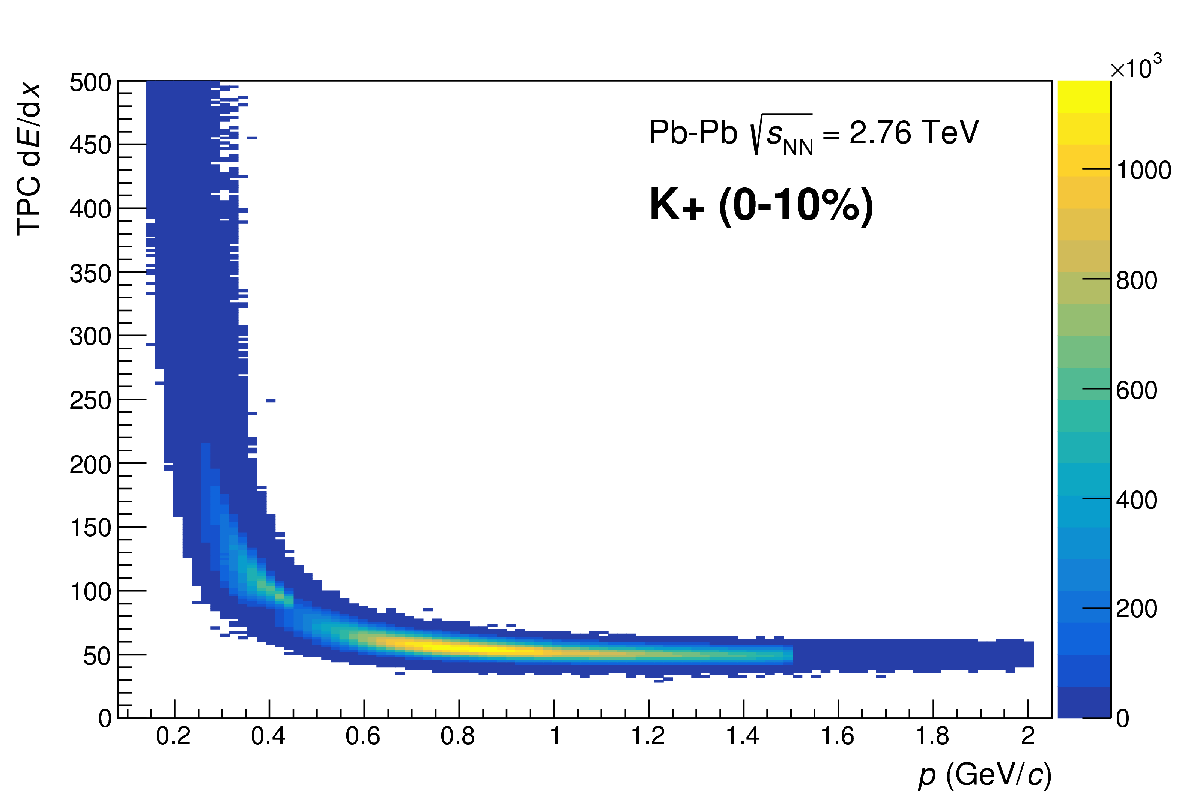
\includegraphics[width=0.5\textwidth]{/home/jesse/Analysis/FemtoAnalysis/LamKPublication/Figures/PDF/canDrawKchdEdx_LamKchP_0010_KchP.pdf}% Here is how to import EPS art
 \caption{\label{fig:KchPdEdx} Sample d$E$/d$x$ distribution for the \KchP collection from our 0-10\% central \LamKchP analysis.}
\end{figure}

\begin{table}[htbp]
 \centering
%  \renewcommand{\arraystretch}{1.5}
  \begin{tabular}{lc|c|l}
   \hline  
   \multicolumn{4}{c}{\textbf{\Kpm selection}} \\
   \hline
   \multicolumn{3}{l|}{Transverse momentum $p_{\mathrm{T}}$} & 0.14 $< p_{\mathrm{T}} < 1.5$ GeV/\textit{c} \\
   \hline
   \multicolumn{3}{l|}{$|\eta|$} & $< 0.8$ \\
   \hline
   \multicolumn{3}{l|}{Transverse DCA to primary vertex} & $<$ 2.4 cm \\
   \hline
   \multicolumn{3}{l|}{Longitudinal DCA to primary vertex} & $<$ 3.0 cm \\
   \hline

   TPC and TOF N$\sigma$ Cuts & \multicolumn{3}{c}{} \\
   \cline{2-4}
    & \multicolumn{1}{l}{$p <$ 0.4 GeV/\textit{c}} &  & N$_{\sigma \mathrm{K,TPC}} <$ 2 \\
   \cline{2-4}
    & \multicolumn{1}{l}{0.4 $< p <$ 0.45 GeV/\textit{c}} & & N$_{\sigma \mathrm{K,TPC}} <$ 1 \\
   \cline{2-4}     
    & \multicolumn{1}{l}{0.45 $< p <$ 0.80 GeV/\textit{c}} & & N$_{\sigma \mathrm{K,TPC}} <$ 3 \\ 
   \multicolumn{3}{c|}{} & N$_{\sigma \mathrm{K,TOF}} <$ 2 \\
   \cline{2-4}
    & \multicolumn{1}{l}{0.80 $< p <$ 1.0 GeV/\textit{c}} & & N$_{\sigma \mathrm{K,TPC}} <$ 3 \\
   \multicolumn{3}{c|}{} & N$_{\sigma \mathrm{K,TOF}} <$ 1.5 \\  
   \cline{2-4}
    & \multicolumn{1}{l}{$p >$ 1.0 GeV/\textit{c}} & & N$_{\sigma \mathrm{K,TPC}} <$ 3 \\
   \multicolumn{3}{c|}{} & N$_{\sigma \mathrm{K,TOF}} <$ 1 \\  
   \hline
   \multicolumn{3}{l|}{\multirow{3}{*}{Electron Rejection: Reject if all satisfied}} & $\mathrm{N}_{\sigma e^{-},\mathrm{TPC}} < $ 3 \\
   \multicolumn{3}{c|}{} & $\mathrm{N}_{\sigma e^{-},\mathrm{TPC}} < \mathrm{N}_{\sigma K^{\pm},\mathrm{TPC}}$ \\
   \multicolumn{3}{c|}{} & $\mathrm{N}_{\sigma e^{-},\mathrm{TOF}} < \mathrm{N}_{\sigma K^{\pm},\mathrm{TOF}}$ \\
   \hline
   
   \multicolumn{4}{l}{Pion Rejection:  Reject if:} \\
   %\cline{1-1}
   \multirow{4}{*}{$p <$ 0.65 GeV/\textit{c}} & \multicolumn{1}{l}{TOF and TPC available} & \multicolumn{1}{c|}{} & N$_{\sigma \pi,\mathrm{TPC}} <$ 3 \\
   \multicolumn{3}{c|}{} & N$_{\sigma \pi,\mathrm{TOF}} <$ 3 \\
   \cline{2-4}
    & \multirow{2}{*}{Only TPC available} & $p <$ 0.5 GeV/\textit{c} & N$_{\sigma \pi,\mathrm{TPC}} <$ 3 \\
   \cline{3-4}
    &  & 0.5 $< p <$ 0.65 GeV/\textit{c} & N$_{\sigma \pi,\mathrm{TPC}} <$ 2 \\
   \cline{2-4}
   \multicolumn{3}{l|}{\multirow{2}{*}{0.65 $< p <$ 1.5 GeV/\textit{c}}} & N$_{\sigma \pi,\mathrm{TPC}} <$ 5 \\
    & \multicolumn{2}{c|}{} & N$_{\sigma \pi,\mathrm{TOF}} <$ 3 \\
   \cline{2-4}
   \multicolumn{3}{l|}{\multirow{2}{*}{$p >$ 1.5 GeV/\textit{c}}} & N$_{\sigma \pi,\mathrm{TPC}} <$ 5 \\
    & \multicolumn{2}{c|}{} & N$_{\sigma \pi,\mathrm{TOF}} <$ 2 \\
   \hline
  \end{tabular}
% \end{minipage}
 \caption{\Kpm selection}
 \label{tab:KchCuts} 
\end{table}

The purity of the \Kpm collections was estimated from a Monte-Carlo (MC) study based on HIJING \cite{PhysRevD.44.3501} simulations using GEANT3 \cite{Brun:1994aa} to model particle transport through the ALICE detectors. 
The charged kaon purity is estimated to be approximately 97\%.
Figure \ref{fig:KchPdEdx} shows a sample d$E$/d$x$ for the \KchP collection in the 0-10\% centrality bin (from our \LamKchP study).



\subsection{\Vz selection}
\label{sec:V0Selection}

\LamALam and \Ks particles are electrically neutral, and cannot be directly detected, but must instead be reconstructed through detection of their decay products, or daughters.  
This process is illustrated in Figure \ref{fig:V0Reconstruction}, and the main cuts used are shown in Tables \ref{tab:LamCuts} and \ref{tab:K0sCuts}.
In general, particles which are topologically reconstructed in this fashion are called \Vz particles.
The decay channel \Lam $\rightarrow$ p$\pi^{-}$ was used for the identification of \Lam hyperons (and, similarly the charge-conjugate decay for the \ALam identification), and \Ks $\rightarrow$ $\pi^{+}\pi^{-}$ for the identification of \Ks mesons.

\begin{figure}[h]
  \centering
  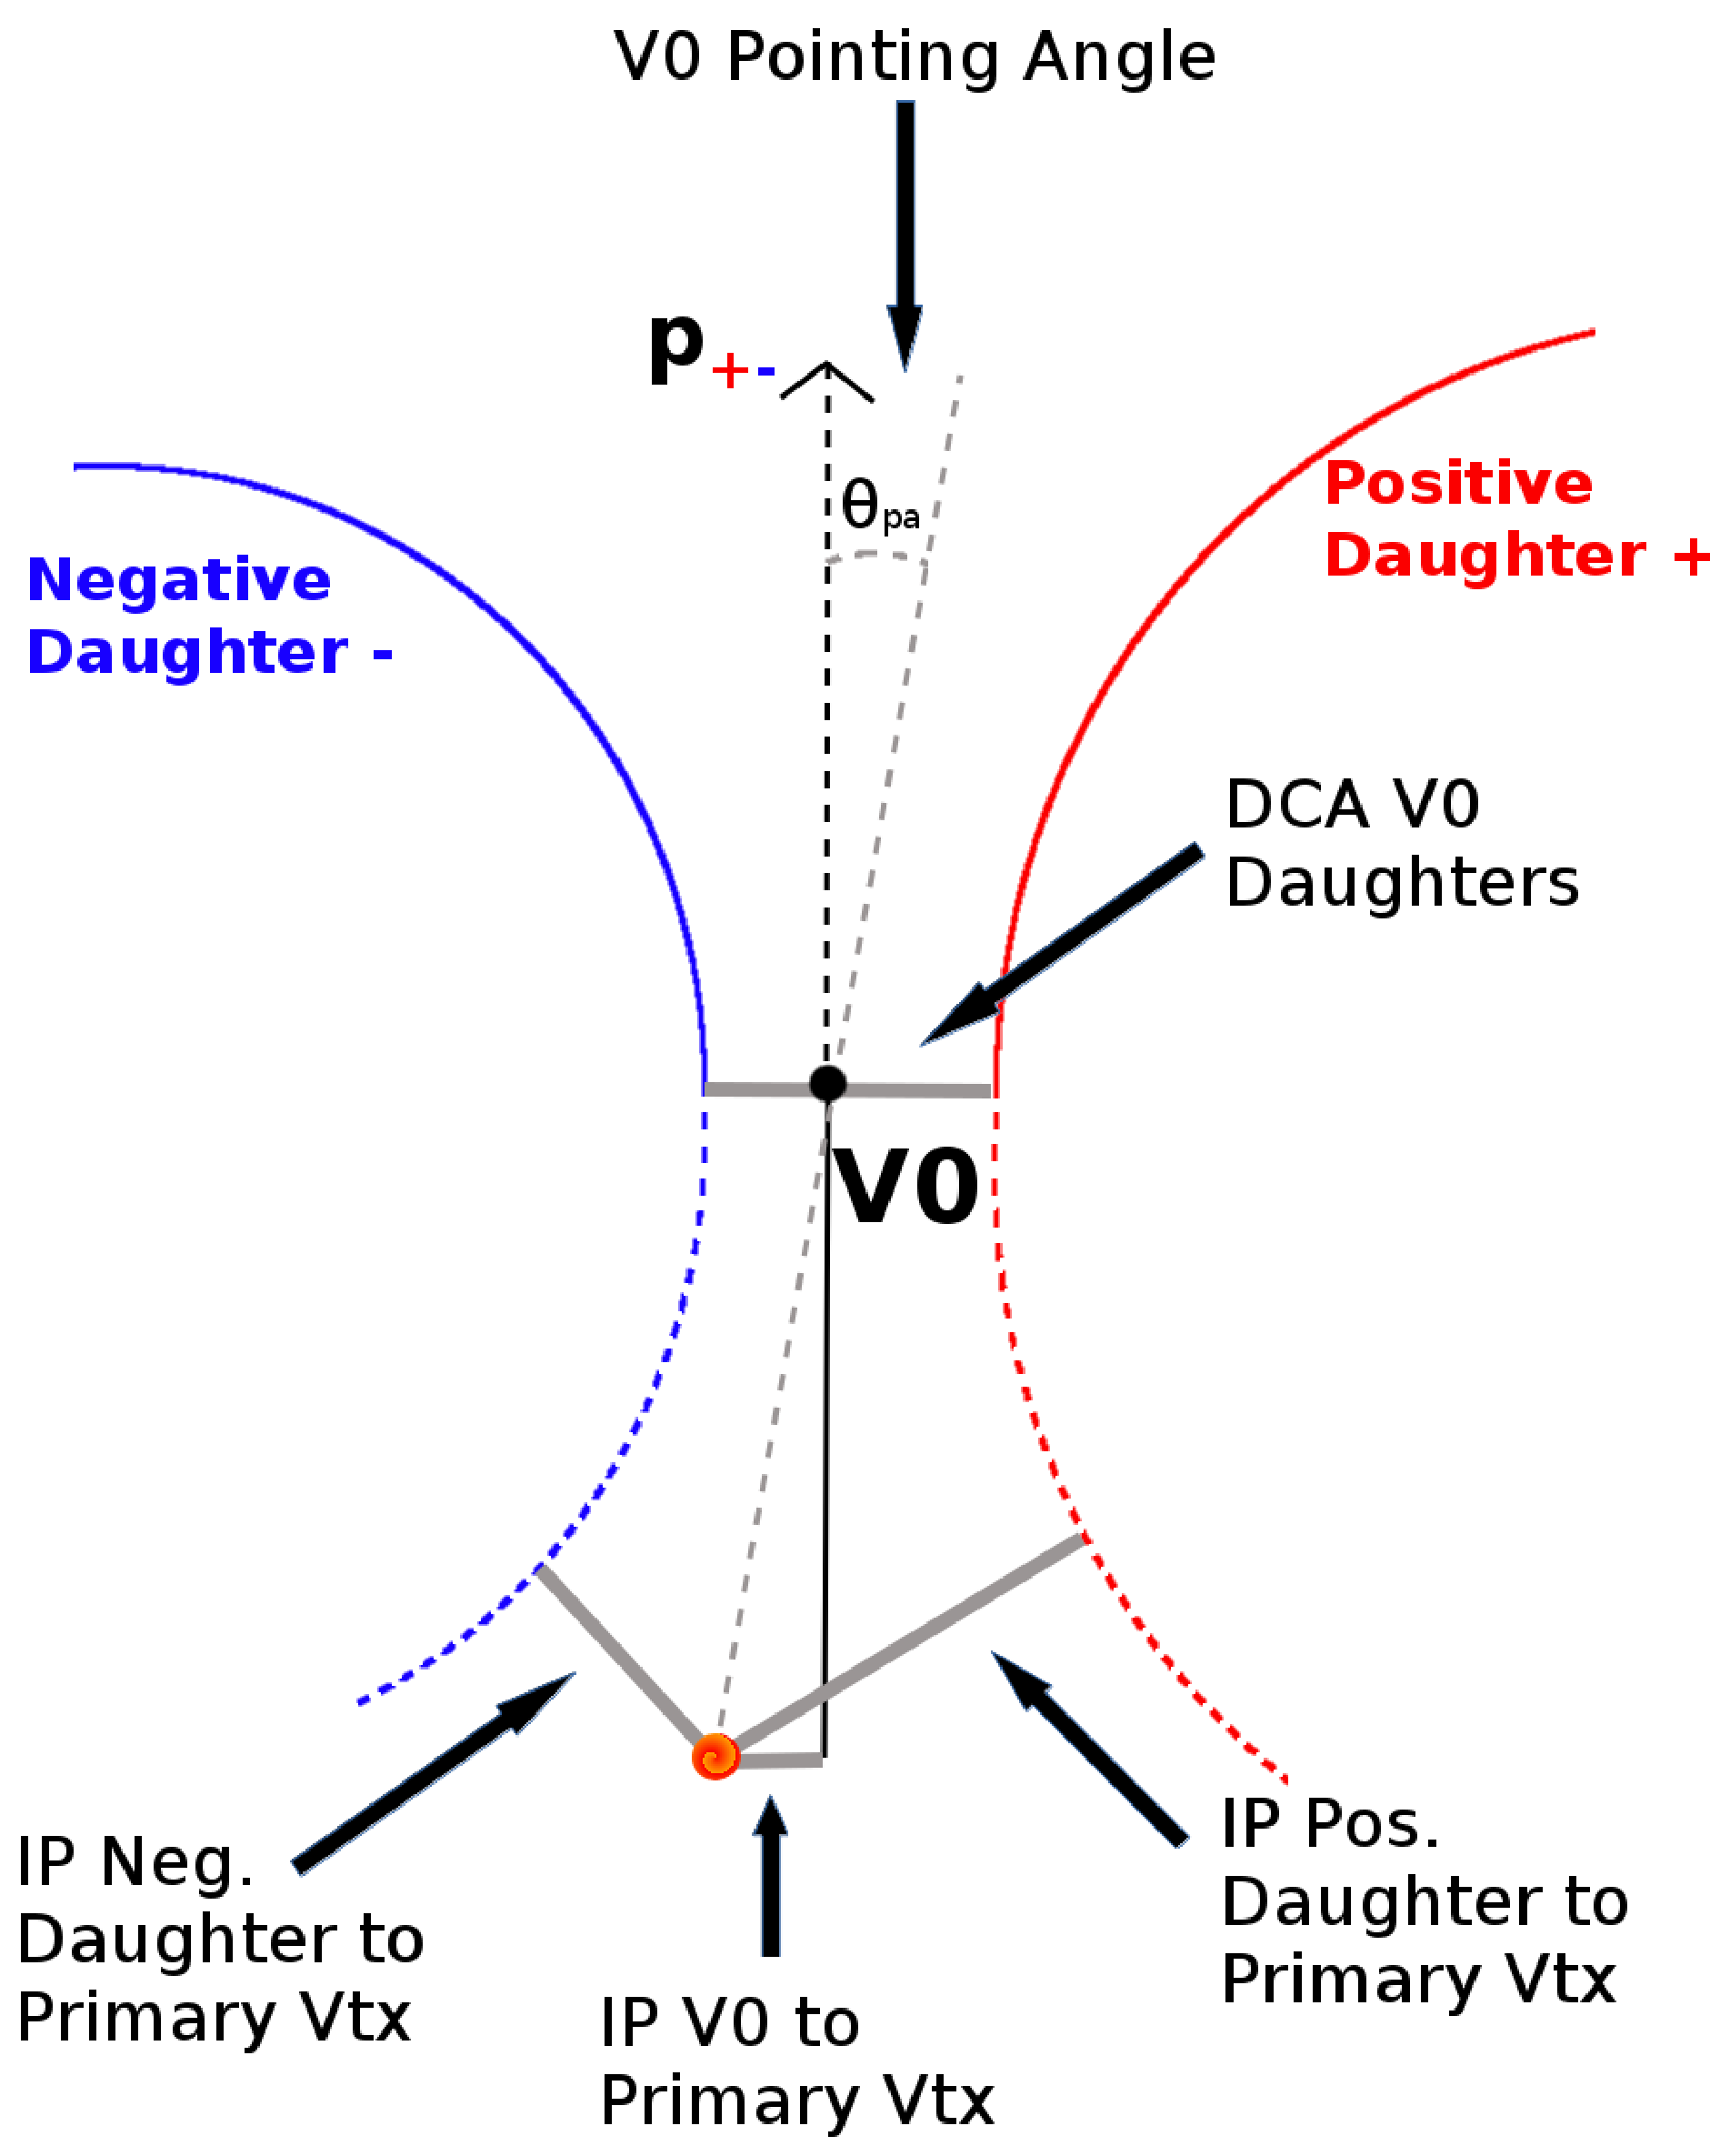
\includegraphics[width=0.30\textwidth]{/home/jesse/Analysis/FemtoAnalysis/LamKPublication/Figures/PDF/V0CutsGeneral.pdf}
  \caption[\Vz Reconstruction]{\Vz Reconstruction}
  \label{fig:V0Reconstruction}
\end{figure}

To construct a \Vz particle, the charged daughter tracks must first be found.  
Aside from typical kinematic and PID cuts (using TPC and TOF detectors), the daughter tracks are also exposed to a minimum cut on their impact parameter with respect to the primary vertex.  
The decay vertex of the \Vz is assumed to be the point of closest approach between the daughter tracks.
To help ensure quality, a maximum value cut is demanded on the distance-of-closest-approach between the daughters (DCA \Vz Daughters).
The positive and negative daughter tracks are combined to form the \Vz candidate, the momentum of which is simply the sum of the momenta of the daughters (calculated at the DCA).

A minimum transverse momentum cut on the \Vz candidate is introduced to reduce contamination from fake candidates.
Opposite to that of the daughter tracks, the \Vz candidate is exposed to a maximum cut on its impact parameter with respect to the primary vertex.
In this case, we do want our \Vz candidates to be primary, hence the maximum cut imposition.
To further strengthen our selection of primary \Vz candidates, we impose a selection on the pointing angle, $\theta_{\mathrm{pa}}$, between the \Vz momentum and the vector pointing from the primary vertex to the secondary \Vz decay vertex, which is achieved by appointing a minimum value on $\cos(\theta_{\mathrm{pa}})$ (``Cosine of pointing angle'' in Tables \ref{tab:LamCuts} and \ref{tab:K0sCuts}).

On occasion, \LamALam particles are misidentified as \Ks, and vice versa.  
To attempt to remove these contaminations without throwing away good candidates, we impose a set of misidentification cuts.  
The intent of these cuts is to judge whether a candidate is more likely a \LamALam or a \Ks, and are implemented as described below.  
For a given \Vz, we calculate the mass assuming different identities (\Lam, \ALam, \Ks) of the candidate; the mass assuming \Ks hypothesis ($m_{\mathrm{inv,~ K^{0}_{S}~ hyp.}}$) is calculated assuming $\pi^{+}\pi^{-}$ daughters, the mass assuming \Lam hypothesis ($m_{\mathrm{inv,~ \Lambda~ hyp.}}$) is calculated assuming p$\pi^{-}$ daughters, and the mass assuming \ALam hypothesis ($m_{\mathrm{inv,~ \bar{\Lambda}~ hyp.}}$) is calculated assuming $\bar{p}\pi^{+}$ daughters.  
In addition to the notation just introduced, in the following, $m_{\mathrm{PDG,~ K^{0}_{S}}}$ and $m_{\mathrm{PDG,~ \Lambda(\bar{\Lambda})}}$ denote the particle masses of the \Ks and \LamALam, respectively, as recorded by the Particle Data Group \cite{Patrignani:2016xqp}.

For \LamALam selection, a candidate is assumed to be misidentified and is rejected if all of the following criteria are satisfied:

\begin{enumerate}
 \item $\left|m_{\mathrm{inv,~ K^{0}_{S}~ hyp.}} - m_{\mathrm{PDG,~ K^{0}_{S}}}\right| < $ 9.0 MeV/$c^{2}$
 \item The daughter particles pass daughter cuts intended for \Ks reconstruction
 \item $\left|m_{\mathrm{inv,~ K^{0}_{S}~ hyp.}} - m_{\mathrm{PDG,~ K^{0}_{S}}}\right|~ < ~\left|m_{\mathrm{inv,~ \Lambda(\bar{\Lambda})~ hyp.}} - m_{\mathrm{PDG,~ \Lambda(\bar{\Lambda})}}\right|$
\end{enumerate} 

Similarly, for \Ks selection, a candidate is rejected if all of the following criteria are satisfied for the \Lam case, or for the \ALam case:

\begin{enumerate}
 \item $\left|m_{\mathrm{inv}, \ \Lambda(\bar{\Lambda}) \ \mathrm{hyp.}} - m_{\mathrm{PDG},\ \Lambda(\bar{\Lambda})}\right| < $ 9.0 MeV/$c^{2}$
 \item The daughter particles pass daughter cuts intended for \LamALam reconstruction
 \item $\left|m_{\mathrm{inv}, \ \Lambda(\bar{\Lambda}) \ \mathrm{hyp.}} - m_{\mathrm{PDG},\ \Lambda(\bar{\Lambda})}\right|~ < ~\left|m_{\mathrm{inv},~ \mathrm{K}^{0}_{S}~ \mathrm{hyp.}} - m_{\mathrm{PDG},~ \mathrm{K}^{0}_{S}}\right|$
\end{enumerate} 

At this stage, we have a collection of \Vz candidates satisfying all of the aforementioned cuts.
However, this collection is still polluted by fake V$^{0}$s, for which the daughter particles happen to pass all of our cuts, but which do not actually originate from a \Vz.
Although the two daughter particles appear to reconstruct a \Vz candidate, they are lacking one critical requirement: the system invariant mass does not match that of our desired \Vz species (these can be seen outside of the mass peaks in Fig. \ref{fig:Purity}).
Therefore, as our final single-particle cut, we require the invariant mass of the \Vz candidate to fall within the mass peak of our desired species.
Note, however, that some fake V$^{0}$s still make it past this final cut, as their invariant mass also happens to fall without our acceptance window.

\begin{table}[htbp]
 \centering 
%  \renewcommand{\arraystretch}{1.5}
  \begin{tabular}{lc|c|l}
   \hline  
   \multicolumn{4}{c}{\textbf{\Lam selection}} \\
   \hline
   \multicolumn{3}{l|}{Transverse momentum $p_{\mathrm{T}}$} & $> 0.4$ GeV/\textit{c} \\
   \hline
   \multicolumn{3}{l|}{$|\eta|$} & $< 0.8$ \\
   \hline
   \multicolumn{3}{l|}{$|m_{\mathrm{inv}} - m_{\mathrm{PDG}}|$} & $< 3.8$ MeV \\ 
   \hline
   \multicolumn{3}{l|}{DCA to primary vertex} & $<$ 0.5 cm \\
   \hline
   \multicolumn{3}{l|}{Cosine of pointing angle} & $>$ 0.9993 \\
   \hline
   \multicolumn{3}{l|}{Decay Length} & $<$ 60 cm \\
   \hline
   
   
   \multicolumn{4}{c}{\textbf{Daughter Cuts ($\pi$ and p)}} \\
   \hline
   \multicolumn{3}{l|}{$|\eta|$} &  $< 0.8$ \\
   \hline
   \multicolumn{3}{l|}{DCA $\pi$p Daughters} & $<$ 0.4 cm \\
   \hline
   
   
   \multicolumn{4}{c}{\textbf{$\pi$-specific cuts}} \\
   \hline
   \multicolumn{3}{l|}{$p_{\mathrm{T}}$} & $> 0.16$ GeV/\textit{c} \\
   \hline
   \multicolumn{3}{l|}{DCA to primary vertex} & $>$ 0.3 cm \\
   \hline
   \multicolumn{4}{l}{TPC and TOF N$\sigma$ Cuts} \\
%   \cline{2-4}
    & \multicolumn{1}{c}{$p <$ 0.5 GeV/\textit{c}} &  & N$\sigma_{\mathrm{TPC}} <$ 3 \\
   \cline{2-4}
    & \multicolumn{1}{c}{\multirow{3}{*}{$p >$ 0.5 GeV/\textit{c}}} &  \multirow{2}{*}{TOF \& TPC available} & N$\sigma_{\mathrm{TPC}} <$ 3 \\
    & \multicolumn{2}{c|}{} & N$\sigma_{\mathrm{TOF}} <$ 3 \\
   \cline{3-4}
    & \multicolumn{1}{c}{} & Only TPC available & N$\sigma_{\mathrm{TPC}} <$ 3 \\
   \hline
   
   
   \multicolumn{4}{c}{\textbf{p-specific cuts}} \\
   \hline
   \multicolumn{3}{l|}{$p_{\mathrm{T}}$} & $ > $ 0.5(p) [0.3($\bar{\mathrm{p}}$)] GeV/\textit{c} \\
   \hline
   \multicolumn{3}{l|}{DCA to primary vertex} & $>$ 0.1 cm \\
   \hline
   \multicolumn{4}{l}{TPC and TOF N$\sigma$ Cuts} \\
   \cline{2-4}
    & \multicolumn{1}{c}{$p <$ 0.8 GeV/\textit{c}} & & N$\sigma_{\mathrm{TPC}} <$ 3 \\
   \cline{2-4}
    & \multicolumn{1}{c}{\multirow{3}{*}{$p >$ 0.8 GeV/\textit{c}}} &  \multirow{2}{*}{TOF \& TPC available} & N$\sigma_{\mathrm{TPC}} <$ 3 \\
    & \multicolumn{2}{c|}{} & N$\sigma_{\mathrm{TOF}} <$ 3 \\
   \cline{3-4}
    & \multicolumn{1}{c}{} & Only TPC available & N$\sigma_{\mathrm{TPC}} <$ 3 \\
   \hline   
  \end{tabular}
% \end{minipage}
 \caption{\Lam selection}
 \label{tab:LamCuts} 
\end{table}



\begin{table}[htbp]
 \centering
%  \renewcommand{\arraystretch}{1.5}
  \begin{tabular}{lc|c|l}
   \hline  
   \multicolumn{4}{c}{\textbf{\Ks selection}} \\
   \hline
   \multicolumn{3}{l|}{Transverse momentum $p_{\mathrm{T}}$} & $> 0.2$ GeV/\textit{c} \\
   \hline
   \multicolumn{3}{l|}{$|\eta|$} & $< 0.8$ \\
   \hline
   \multicolumn{4}{l}{$m_{PDG}-13.677 \ \mathrm{MeV} < m_{\mathrm{inv}} < m_{\mathrm{PDG}} + 2.0323 \ \mathrm{MeV}$} \\ 
   \hline
   \multicolumn{3}{l|}{DCA to primary vertex} & $<$ 0.3 cm \\
   \hline
   \multicolumn{3}{l|}{Cosine of pointing angle} & $>$ 0.9993 \\
   \hline
   \multicolumn{3}{l|}{Decay Length} & $<$ 30 cm \\
   \hline
      
   
   \multicolumn{4}{c}{\textbf{$\pi^{\pm}$ Daughter Cuts}} \\
   \hline
   \multicolumn{3}{l|}{$p_{\mathrm{T}}$} & $>$ 0.15 GeV/\textit{c} \\
   \hline
   \multicolumn{3}{l|}{$|\eta|$} &  $< 0.8$ \\
   \hline
   \multicolumn{3}{l|}{DCA $\pi^{+}\pi^{-}$ Daughters} & $<$ 0.3 cm \\
   \hline
   \multicolumn{3}{l|}{DCA to primary vertex} & $>$ 0.3 cm \\
   \hline
   \multicolumn{4}{l}{TPC and TOF N$\sigma$ Cuts} \\
%   \cline{2-4}
    & \multicolumn{1}{c}{$p <$ 0.5 GeV/\textit{c}} &  & N$\sigma_{\mathrm{TPC}} <$ 3 \\
   \cline{2-4}
    & \multicolumn{1}{c}{\multirow{3}{*}{$p >$ 0.5 GeV/\textit{c}}} &  \multirow{2}{*}{TOF \& TPC available} & N$\sigma_{\mathrm{TPC}} <$ 3 \\
    & \multicolumn{2}{c|}{} & N$\sigma_{\mathrm{TOF}} <$ 3 \\
   \cline{3-4}
    & \multicolumn{1}{c}{} & Only TPC available & N$\sigma_{\mathrm{TPC}} <$ 3 \\
   \hline   
  \end{tabular}
% \end{minipage}
 \caption{\Ks selection}
 \label{tab:K0sCuts} 
\end{table}

Occasionally, we encounter a situation where two \Vz candidates share a common daughter.
Not both of these candidates can be real V$^{0}$s, and including both could introduce an artificial signal into our data.
To avoid any auto-correlation effects, for each event, we impose a single-particle shared daughter cut on each collection of \Vz candidates.
This cut iterates through the \Vz collection to ensure that no daughter is claimed by more than one \Vz candidate.
If a shared daughter is found between two \Vz candidates, that candidate with a smaller DCA to primary vertex is kept while the other is excluded from the analysis.
Note, this single-particle shared daughter cut is unique from the pair shared daughter cut discussed in Sec. \ref{PairConstruction}, the latter of which ensure there is no daughter sharing between the particles in a given pair.

In order to obtain a true and reliable signal, one must ensure good purity of the \Vz collection.  The purity of the collection is calculated as:

\begin{equation}
 Purity = \frac{Signal}{Signal + Background}
\label{eqn:Purity}
\end{equation}

To access both the signal and background, the invariant mass distribution (\minv) of all \Vz candidates must be constructed immediately before the final invariant mass cut, as shown in Fig. \ref{fig:Purity} for \Lam and \Ks candidates in the 0-10\% centrality bin.
Figure \ref{fig:Purity:a} presents the p$\pi^{-}$ invariant mass distribution showing the \Lam peak, and Figure \ref{fig:Purity:b} presents the $\pi^{+}\pi^{-}$ invariant mass distribution showing the \Ks peak.
These distributions (and similar for \ALam) are used to calculate the collections' purities (defined in Eq. \ref{eqn:Purity}).
As shown in Figure \ref{fig:Purity}, the background is fit (with a polynomial) outside of the peak region of interest to obtain an estimate for the background within the region.
Within the \minv cut limits, the background is assumed to be the region below the fit while the signal is that above the fit.
The \Lam and \ALam purities were found to be $\approx$ 95\%, and the \Ks purity was found to be $\approx$ 98\%.

\begin{figure}[htp]
  \centering
  %%----start of first subfigure---
  \subfigure[p$\pi^{-}$ invariant mass distribution where the \Lam peak is seen.]{
    \label{fig:Purity:a}
    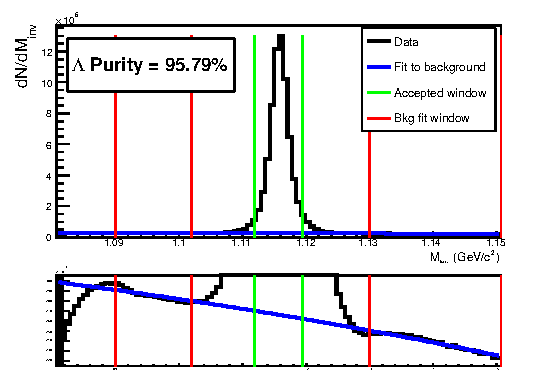
\includegraphics[width=0.49\linewidth]{/home/jesse/Analysis/FemtoAnalysis/LamKPublication/Figures/PDF/LamPurity_LamK0.pdf}}
  %%----start of second subfigure---  
  \subfigure[$\pi^{+}\pi^{-}$ invariant mass distribution where the \Ks peak is seen.]{
    \label{fig:Purity:b}
    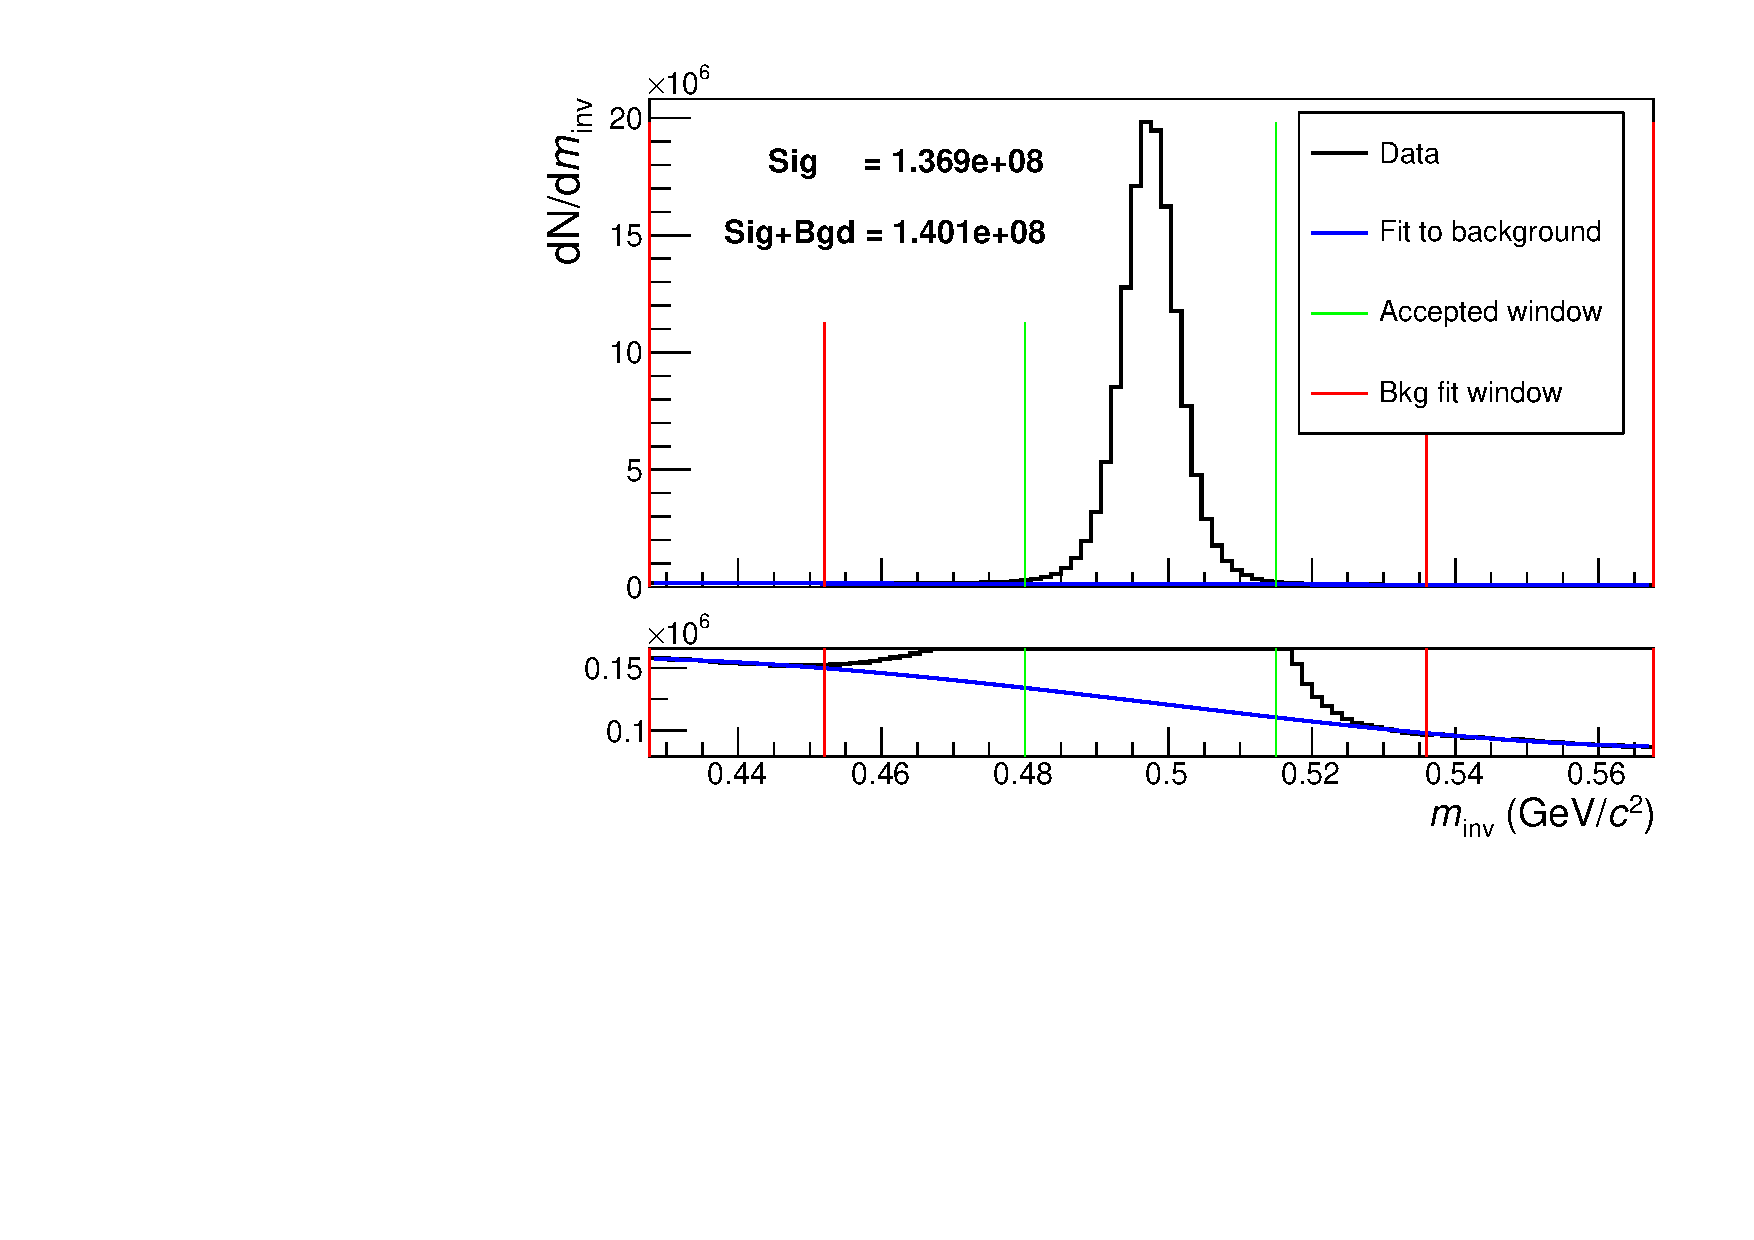
\includegraphics[width=0.49\linewidth]{/home/jesse/Analysis/FemtoAnalysis/LamKPublication/Figures/PDF/K0Purity_LamK0.pdf}}
  %%----overall caption----
  \caption{Invariant mass (\minv) distribution of p$\pi^{+}$ pairs showing the \Lam peak \ref{fig:Purity:a}, and of $\pi^{+}\pi^{-}$ pairs showing the \Ks peak \ref{fig:Purity:b}, for \Vz candidates.  The bottom panels are zoomed to show the background with fit.  The vertical green lines represent the \minv cuts used in the analyses, the red vertical lines delineate the region over which the background was fit, and the blue line shows the background fit.}  
  \label{fig:Purity}
\end{figure}






\subsection{Pair Construction}
\label{PairConstruction}


In order to reduce the contamination to the two-particle correlations due to split or merged tracks and pairs sharing daughters, two main pair cuts are applied: a shared daughter cut, and an average separation cut.
The purpose of the shared daughter cut is to ensure the first particle in the pair is unique from the second.  
For pairs formed of two V$^{0}$s (i.e. \LamKs), this cut is implemented by removing all pairs which share a daughter.  
For a pair formed of a single \Vz and a charged track (i.e. \LamKpm), the cut removes all pairs in which the charged track is also claimed as a daughter of the \Vz.  


The purpose of the average separation cut is to remove splitting and merging effects, and it is employed in the following way.  
To calculate the average separation between two tracks, the spatial separation is determined at several points throughout the TPC (every 20 cm radially from 85 cm to 245 cm), and the results averaged.
For that \LamKs analysis, which involves two \Vz particles, a minimum average separation cut of 6 cm between the like-charge daughters in the pairs was imposed (for example, between the p daughter of the \Lam and the $\pi^{+}$ daughter of the \Ks).
For the \LamKpm analyses, a minimum average separation cut of 8 cm was enforced between the \Kpm and the \Lam daughter sharing the same charge (for example, in the \LamKchP analysis, between the p daughter of the \Lam and the \KchP).
The values used in these cuts were obtained by first forming average separation correlation functions.
This is done just as for our relative-momentum correlation functions, but we instead bin in average separation.
Looking at these average separation correlation functions for like-charge tracks, at lowest average separation we see an enhancement due to track splitting, followed by (at slightly higher average separation) a suppression due to track merging.
When the average separation correlation function stabilizes to unity, these effects are no longer abundant, and we choose our cut value.
Splitting and merging effects between oppositely charged tracks was found to be negligible, therefore no cuts on unlike-charge tracks were imposed.



\section{Analysis Methods}
\label{sec:AnalysisMethods}

\subsection{Correlation Function}
\label{sec:CorrelationFunction}
Two-particle correlation functions are built as the ratio of the covariant two-particle and single-particle spectra:

\begin{equation}
  C^{ab}(\vec{\mathrm{p}_{a}},\vec{\mathrm{p}_{b}}) = \frac{E_{a}E_{b}\frac{dN^{ab}}{d^{3}p_{a}d^{3}p_{b}}}{\big( E_{a}\frac{dN^{a}}{d^{3}p_{a}} \big) \big( E_{b}\frac{dN^{b}}{d^{3}p_{b}} \big)}
\label{eqn:CfRatioSpectra}
\end{equation}

This may be expressed theoretically as in the Koonin-Pratt equation \cite{Koonin:1977fh, Pratt:1990zq}:

\begin{equation}
 C(\mathbf{k^{*}}) = \int S_{\mathbf{P}}(\mathbf{r^{*}})|\Psi_{\mathbf{k^{*}}}(\mathbf{r^{*}})|^{2}d^{3}\mathbf{r^{*}}
\label{eqn:KooninPrattEqn}
\end{equation}

where $\mathbf{k}^{*}$ is the relative momentum of the pair (defined as $\mathbf{k}^{*} = \frac{1}{2}|\mathbf{p}_{1}^{*}-\mathbf{p}_{2}^{*}|$, where $\mathbf{p}_{1}^{*}$ and $\mathbf{p}_{2}^{*}$ are the momenta of the two particles) in the pair rest frame (PRF), $\mathbf{r}^{*}$ is the relative separation in the same frame, $\mathbf{P}$ is the total pair momentum, $S_{\mathbf{P}}(\mathbf{r^{*}})$ is the pair source distribution, and $\Psi_{\mathbf{k^{*}}}(\mathbf{r^{*}})$ is the two-particle wave-function.
Within the $|\Psi|^{2}$ term is contained the particle interaction information, and therefore the scattering parameters.
Equation \ref{eqn:KooninPrattEqn} reveals the limitations of femtoscopy; at best, we are able to probe the distribution of relative positions of particles with identical velocities and total momentum $\mathbf{P}$ as they move in an asymptotic state.  
Therefore, we do not measure the entire size of the source, but rather the ``regions of homogeneity'' \cite{Akkelin:1995gh}.

In practice, the correlation function is formed experimentally as:

\begin{equation}
  C(k^{*}) = \mathcal{N}\frac{A(k^{*})}{B(k^{*})}
\label{eqn:CfExp}
\end{equation}


where $A(k^{*})$ is the signal distribution, $B(k^{*})$ is the reference distribution, and $\mathcal{N}$ is a normalization parameter.  
$B(k^{*})$ is used to divide out the phase-space effects, leaving only the femtoscopic effects in the correlation function. 
The normalization parameter is chosen such that the mean value of the correlation function equals unity for \kstar $\in$ [0.32, 0.4] GeV/$c$.


In practice, $A(k^{*})$ is constructed by binning in \kstar pairs from the same event.
Typically, $B(k^{*})$ is obtained by forming mixed-event pairs, i.e. particles from a given event are paired with particles from $\rm N_{mix}$ other events, and these pairs are then binned in \kstar.
Other techniques exist; most notably, one may use same-event pairs after rotating one particle in the pair by 180$^\circ$ in the transverse plane (see Sec. \ref{NonFlatBackground} and App. \ref{App:StavMethod} for more details).
However, for this analysis, we use the typical mixed-event method.
In order to mix only similar events, we bin our events both in primary vertex location (2 cm bin width) and in centrality (5\% bin width), and we only mix events within a given bin; i.e. we only mix events of like centrality and of like primary vertex location.
Additionally, we use $\rm N_{mix} = 5$ as the size of our mixing pool.
Also note, a vertex correction is also applied to each event, which essentially recenters the the primary vertices to z = 0.


This analysis presents correlation functions for three centrality bins (0-10\%, 10-30\%, and 30-50\%), and is currently pair transverse momentum ($k_{\mathrm{T}} = \frac{1}{2}|\mathbf{p}_{\mathrm{T,1}}+\mathbf{p}_{\mathrm{T,2}}|$) integrated (i.e. not binned in $k_{\mathrm{T}}$).  
The correlation functions are constructed separately for the two magnetic field configurations ($++$ and $--$).
These are kept separate during the fitting process, and are combined using a weighted average when plotting, where the weight is the number of numerator pairs in the normalization range.

\subsection{Modeling the correlation function}
\label{sec:ModelingCF}


In the absence of the Coulomb interaction, the correlation function can be described analytically with a model derived by Lednick\'y and Lyuboshitz \cite{Lednicky:82}.
Within the model, the (non-symmetrized) two-particle wave function is expressed as a superposition of a plane wave and diverging spherical wave:

\begin{equation}
\begin{aligned}
\Psi^{S}(\mathbf{k}^{*}, \mathbf{r}^{*}) = e^{-i\mathbf{k}^{*} \cdot \mathbf{r}^{*}} + f^{S}(k^{*})\frac{e^{ik^{*}r^{*}}}{r^{*}}
\end{aligned}  
\label{eqn:NonSymmPsi}
\end{equation}

In the effective range approximation, the complex s-wave scattering amplitude, $f^{S}(k^{*})$, with $S$ denoting the total spin of the particular pair, is of the form

\begin{equation}
\begin{aligned}
f^{S}(k^{*}) = \left( \frac{1}{f^{S}_{0}} + \frac{1}{2}d^{S}_{0}k^{*2} - ik^{*} \right)^{-1}
\end{aligned}
\label{eqn:ScatteringParam}
\end{equation}

where $f^{S}_{0}$ is the complex s-wave scattering length, and $d^{S}_{0}$ is the effective range of the interaction.
A spherically symmetric Gaussian distribution with radius $R_{\mathrm{inv}}$  is assumed for the pair emission source in the PRF.
Assuming unpolarized emission, using the appropriately symmetrized form of $\Psi$ (Eq. \ref{eqn:NonSymmPsi}) with a spherically symmetric Gaussian source (Eq. \ref{eqn:GaussianSource}), with the Koonin-Pratt equation (Eq. \ref{eqn:KooninPrattEqn}), the correlation function for uncharged particles is given by \cite{Lednicky:82}

\begin{equation}
 C(k^{*}) = 1 + C_{\mathrm{QI}}(k^{*}) + C_{\mathrm{FSI}}(k^{*})
\label{eqn:LednickyEqn}
\end{equation}

$C_{\mathrm{QI}}$ describes plane-wave quantum interference:

\begin{equation}
 C_{\mathrm{QI}}(k^{*}) = \alpha\exp(-4k^{*2}R^{2})
\label{eqn:CQI}
\end{equation}

where $\alpha = (-1)^{2j}/(2j+1)$ for identical particles with spin j, and $\alpha = 0$ for non-identical particles.   
$C_{\mathrm{FSI}}$ describes the s-wave strong final state interaction between the particles:



\begin{equation}
\begin{aligned}
C_{\mathrm{FSI}}(k^{*}) &= \sum_{S}\rho_{S}\left[\frac{1}{2}\left|\frac{f^{S}(k^{*})}{R_{\mathrm{inv}}}\right|^2\left(1-\frac{d^{S}_{0}}{2\sqrt{\pi}R_{\mathrm{inv}}}\right)+\frac{2\Re f^{S}(k^{*})}{\sqrt{\pi}R_{\mathrm{inv}}}F_{1}(2k^{*}R_{\mathrm{inv}})-\frac{\Im f^{S}(k^{*})}{R_{\mathrm{inv}}}F_{2}(2k^{*}R_{\mathrm{inv}})\right]
\end{aligned}  
\label{eqn:CFSI}
\end{equation}

where 
\begin{equation}
F_{1}(z) = \int_{0}^{z} \frac{e^{x^{2}-z^{2}}}{z}dx; \qquad
F_{2}(z) = \frac{1-e^{-z^{2}}}{z}
\label{eqn:CFSI2}
\end{equation}

The weight factor, $\rho_{S}$ is the normalized emission probability for a state of total spin $S$; in the assumed case of unpolarized emission, $\rho_{S} = (2S+1)/[(2j_{1}+1)(2j_{2}+1)]$, where $j_{1,2}$ are the spins of the particles in the pair.

An additional parameter $\lambda$ is typically included in the femtoscopic fit function to account for the purity of the pair sample, as well as the presence of any uncorrelated pairs.  
In the case of no residual correlations (to be discussed in Section \ref{ResidualCorrelations}), the fit function becomes:

\begin{equation}
 C(k^{*}) = 1 + \lambda[C_{\mathrm{QI}}(k^{*}) + C_{\mathrm{FSI}}(k^{*})]
\label{eqn:LednickyEqnwLambda}
\end{equation}

The presented formalism simplifies for the \LamK system.
The particles in the pairs are obviously non-identical, therefore $\alpha=0$, and we need not worry about the quantum statistical term, $C_{\mathrm{QI}}$.
Furthermore, \Lam is spin-1/2 and K are spin-0, so the \LamK system only has one possible total spin state $S$, and therefore $C_{\mathrm{FSI}}$ has only a single term.
In the following, we drop the $S$ superscript from all scattering parameters.

\subsection{Residual Correlations}
\label{ResidualCorrelations}

The purpose of this analysis is study the interaction and scale of the emitting source of the primary \LamK pairs.
In order to obtain correct results, it is desirable for our particle collections to consist of primary particles.
In practice, this is impossible to achieve; many of our particles are not primary, but originate as decay products from other resonances.
Some of our \Lam hyperons decay from $\Sigma^{0}$, $\Xi^{0}$, $\Xi^{-}$ and $\Sigma^{*(+,-,0)}(1385)$ parents, and some of our K mesons decay from K$^{*(+,-,0)}(892)$ parents.
In these decays, the daughter carries away a momentum very similar to that of its parent.
As a result, the correlations between the particles in the daughter pair will be sensitive to, and dependent upon, the interaction between the parents.
In effect, the correlation between the parents will be visible, although smeared out, in the daughters' signal.
We call this a residual correlation resulting from feed-down.  

The finally measured correlation function is a combination of the genuine \LamK correlation with contributions from residual feed-down and misidentified particles

\begin{eqnarray}
\label{eqn:Residuals} 
 C_{\mathrm{measured}}(k^{*}_{\Lambda\mathrm{K}}) &=& 1 + \lambda'_{\Lambda\mathrm{K}}[C_{\Lambda\mathrm{K}}(k^{*}_{\Lambda\mathrm{K}}) - 1] + \sum\limits_{i,j}  \lambda'_{ij}[C_{ij}(k^{*}_{\Lambda\mathrm{K}})-1] \\
 \lambda_{ij}' &=& \lambda_{\mathrm{Fit}}\lambda_{ij} \notag \\
 \sum\limits_{i,j}\lambda_{ij}' &=&  \lambda_{\mathrm{Fit}}\sum\limits_{i,j}\lambda_{ij} = \lambda_{\mathrm{Fit}} \notag
\label{eqn:CfwRes} 
\end{eqnarray}

where the \LamK term represents the genuine \LamK correlation, and the $i$, $j$ terms denote the contributions from residual feed-down and possible impurities.
More specifically, $C_{ij}(k^{*}_{\Lambda\mathrm{K}})$ is the correlation function between parents of particle species $i$ and $j$, expressed in the basis of the relative momentum of the observed daughter \LamK pairs.  
The $\lambda$ parameters serve as weight dictating the strength of the parent contribution to the daughter pair, and are normalized to unity.
The individual $\lambda_{ij}$ are fixed (and whose values can be found in Table \ref{tab:LambdaValues_All}), but the parameter $\lambda_{\mathrm{Fit}}$ is left free.
The $\lambda_{\mathrm{Fit}}$ parameter serves as an overall normalization shared by all contributors.

In order to obtain the parent correlation function expressed in the relative momentum of the daughter pair, one must use a transform matrix.
The transform matrix describes the decay kinematics of the parent system into the daughter, and maps the \kstar of the parent pair onto that of the daughter.
Using this matrix, the transformed residual correlation function can be obtained:


\begin{equation}
  C_{ij}(k^{*}_{\Lambda\mathrm{K}}) \equiv \frac{\sum\limits_{k^{*}_{ij}} C_{ij}\left(k^{*}_{ij}\right) T\left(k^{*}_{ij},k^{*}_{\Lambda\mathrm{K}}\right)}{\sum\limits_{k^{*}_{ij}} T\left(k^{*}_{ij},k^{*}_{\Lambda\mathrm{K}}\right)}
\label{eqn:ResidualsTransform}
\end{equation}


The transform matrix is generated with the THERMINATOR 2 \cite{Chojnacki:2011hb} simulation. 
It is formed for a given parent pair, $ij$, by taking all \LamK pairs originating from $ij$, calculating the relative momentum of the parents ($k^{*}_{ij}$) and daughters ($k^{*}_{\Lambda\mathrm{K}}$), and filling a two-dimensional histogram with the values. 
The transform matrix is essentially an unnormalized probability distribution mapping the \kstar of the parent pair to that of the daughter pair when one or both parents decay.

Femtoscopic analyses are sensitive to the pair emission structure at kinetic freeze-out.
Therefore, in the eyes of femtoscopy, any particle born from a resonance decay before last rescattering is seen as primary.
For our study, when including three residual contributors, we consider a particle to be primary if its parent has a proper decay length of $c\tau <$ 10 fm.
When including ten residual contributors, we must reduce this number to $c\tau <$ 4 fm for consistency.
Moving to ten contributors, we introduce feed-down from $\Sigma^{*}$ and K$^{*}$ resonances, with proper decay lengths of $c\tau \approx$ 5 fm and $c\tau \approx$ 4 fm, respectively.
As these are considered non-primary for the case of ten contributors, so must any resonance with $c\tau >$ 4 fm.

 
As previously stated, the $\lambda$ parameters dictate the strength of the parent contribution to the daughter pair.  
Therefore, the $\lambda$ parameter for parent system AB can be estimated as the total number of $\Lambda$K pairs in our experimental sample originating from AB (N$_{AB}$) divided by the total number of $\Lambda$K pairs (N$_{Total}$):

\begin{equation}
\lambda_{AB} = \frac{N_{AB}}{N_{Total}}
\end{equation}

The particle yields can be estimated using THERMINATOR 2 simulation ($N_{ij}^{\scaleto{THERM}{3pt}}$), while the reconstruction efficiencies ($RE_{ij}$) are estimated with MC HIJING data, which has been run through GEANT to simulate the detector response.  Thus, the $\lambda$ parameters are estimated as:

\begin{equation}
\lambda_{AB} = \frac{N_{AB}}{N_{Total}} = \frac{N_{AB}^{\scaleto{THERM}{3pt}}RE_{AB}^{\scaleto{HIJING}{3pt}}}{\sum\limits_{ij} N_{ij}^{\scaleto{THERM}{3pt}}RE_{ij}^{\scaleto{HIJING}{3pt}}}
\end{equation}

The $\lambda$ values used can be found in Table \ref{tab:LambdaValues_All}, for the case of both three and ten residual contributors.  In the table, we also list the $\lambda$ values used for ``Other'' and ``Fakes''.  The ``Other'' category contains pairs which are not primary, and which do not originate from the (3 or 10) residual pairs included in the fit.  The ``Fakes'' category represents pairs that are mistakenly identified as \LamK.  To estimate this $\lambda_{\mathrm{Fakes}}$ value, we assumed that the number of fake pairs was equal to the total number of pairs multiplied by the \Lam purity (i.e. assuming perfect purity for the kaons); or, more simply, $\lambda_{\mathrm{Fakes}}$ = 1.0 - Purity(\Lam).  For both of these contributors (``Other'' and ``Fakes''), we assume that these correlations average to unity, and therefore do not contribute to the final correlation function.

In practice, we model the correlation function of the parents (e.g. $\Sigma^{0}$\KchP), and run the correlation function through the appropriate transform matrix to determine the contribution to the daughter correlation function (e.g. \LamKchP).  
In an ideal world, we would simply look up the parent interaction in some table, and input this into our model, and form the parent correlation function, $C_{ij}$.  
Unfortunately, the world in which we live is not perfect, such a table does not exists, and little is know about the interaction between the particles in the residual pairs of this study. 
Additionally, introducing a unique set of scattering parameters and radii for each residual system would introduce a large number of additional fit parameters, for which we do not have many constraints, and would cause our fitter to be too unconstrained and yield untrustworthy results. 
For this analysis, we assume all residual pairs have the same source size as the daughter pair.
Furthermore, we assume Coulomb-neutral residual pairs share the same scattering parameters as the daughter pair.
Therefore, for Coulomb-neutral pairs, such as $\Sigma^{0}$K, and $\Xi^{0}$K, $C_{ij}(k^{*}_{ij})$ is calculated from Eqn. \ref{eqn:LednickyEqn}, with the help of Eqn. \ref{eqn:CFSI}; $C_{ij}(k^{*}_{\Lambda\mathrm{K}})$ is then obtained by transforming $C_{ij}(k^{*}_{ij})$ with Eq. \ref{eqn:ResidualsTransform}, using the appropriate transform matrix.  

For residual pairs affected by both the strong and Coulomb interactions, things are a bit more complicated.
This is due to the fact that, for the case of both strong and Coulomb interaction, we no longer have a nice analytical form with which to fit.
Generating a correlation function including both is also time consuming, as described further in Appendix \ref{App:CoulombFitter}.
When modeling \XiKpm residual correlations, we use the experimental \XiKpm data; in this case, there is no need to make any assumptions about scattering parameters or source sizes. 
For the other cases, we assume the strong interaction is negligible, and generate the parent correlation assuming a Coulomb-only scenario (see Appendix \ref{App:CoulombFitter} for more details).
This approximation is well justified here as a Coulomb-only description of the system describes, reasonably well, the broad features of the correlation; the strong interaction is necessary for the fine details.  
However, as these correlations are run through a transform matrix, which largely flattens out and fine details, a Coulomb-only description should be sufficient.  
This is reinforced by the fact that we find consistent results between using the $\Xi$K data and the Coulomb-only model of the $\Xi$K data in our treatment of the residual contribution.  


\subsection{Momentum Resolution Corrections}
\label{MomentumResolutionCorrections}

Finite track momentum resolution causes the reconstructed momentum of a particle to smear around the true value.
This, of course, also holds true for \Vz particles.
The effect is propagated up to the pairs of interest, which causes the reconstructed relative momentum (\krec) to differ from the true momentum (\ktrue).
Smearing of the momentum typically will result in a suppression and broadening of the signal.


The effects of finite momentum resolution can be investigated using the MC data, for which both the true and reconstructed momenta are available.
Information gained from looking at \krec vs \ktrue can be exploited to generate response matrices.
A response matrix describes quantitatively how each \krec bin receives contributions from multiple \ktrue bins, and can be used to account for the effects of finite momentum resolution.
With this approach, the resolution correction is applied on-the-fly during the fitting process by propagating the theoretical (fit) correlation function through the response matrix, according to:  

\begin{equation}
  C_{\mathrm{fit}}(k^{*}_{\mathrm{Rec}}) = \dfrac{\sum\limits_{k^{*}_{\mathrm{True}}}M_{k^{*}_{\mathrm{Rec}},k^{*}_{\mathrm{True}}}C_{\mathrm{fit}}(k^{*}_{\mathrm{True}})}{\sum\limits_{k^{*}_{\mathrm{True}}}M_{k^{*}_{\mathrm{Rec}},k^{*}_{\mathrm{True}}}}
\label{eqn:MomResCorrection}
\end{equation}

where $M_{k^{*}_{\mathrm{Rec}},k^{*}_{\mathrm{True}}}$ is the response matrix, $C_{\mathrm{fit}}(k^{*}_{\mathrm{True}})$ is the fit binned in \ktrue, and the denominator normalizes the result.
Equation \ref{eqn:MomResCorrection} describes that, for a given \krec bin, the observed value of $C(k^{*}_{\mathrm{Rec}})$ is a weighted average of all $C(k^{*}_{\mathrm{True}})$ values, where the weights are the normalized number of counts in the [\krec, \ktrue] bin.



\subsection{Non-Flat Background}
\label{NonFlatBackground}

We observe a significant non-femtoscopic, non-flat, background in all of our correlations at large \kstar.  
This background increases with decreasing centrality, is the same amongst all \LamKpm pairs, and is more pronounced in the \LamKs system.
This difference in \LamKpm and \LamKs backgrounds is due mainly to the difference in kinematic cuts, not due to any interesting physics.  

It is suggested that this background effect is due primarily to particle collimation associated with elliptic flow \cite{Kisiel:2017}.  
More specifically, these backgrounds result from mixing events with unlike event-plane angles ($\Psi_{\textrm{EP}}$).  
As explained in \cite{Kisiel:2017}, when elliptic flow is present, all particles are more likely to be emitted in a specific direction (in-plane), as opposed to a perpendicular direction.  
Therefore, the difference in momenta for pairs of particles tends to be smaller, compared to the case of no flow.  
In the case of mixed-event pairs, the two events used do not share an event-plane, and therefore there is no collimation effect in the pairs from flow.  
As a result, pairs with larger momentum are more likely when mixed-events are used (in the denominator of the correlation function), causing the correlation function to dip below unity.  
This same reasoning suggests that the background should lead to an enhancement at low-$k^{*}$. 

The issue here is that we need to know the behavior of the non-femtoscopic background in the low-\kstar region, but we only cleanly observe it in the region further out where there is no femtoscopic signal.
Unfortunately, we cannot simply rotate each event to artificially align their event-planes and rid ourselves of this mixing effect, as our azimuthal angle acceptance is not perfectly uniform, and we have only finite event-plane resolution.
With better resolution, one could simply bin events in $\Psi_{\mathrm{EP}}$ and only mix events within a given bin.
We pursued this direction, and observed a slight decrease in the background; however, going to finer binning, we saw no additional reduction in the background, signaling that we had reached the limits dictated by the resolution.
In the end, we are forced to model the background to include it into our fit.

THERMINATOR 2 simulation has been shown to reproduce the background features in a $\pi$K analysis \cite{Kisiel:2017}.  
After issuing each simulated event a random $\Psi_{\mathrm{EP}}$, we found THERMINATOR 2 did an exceptional job of describing our data.  
Furthermore, the simulation showed the non-femtoscopic background affects the correlation function as a separable scale factor.
Figure \ref{fig:BgdswTHERM} shows the THERMINATOR 2 simulation (gold) together with experimental data (red, blue, or black).  
The figure also shows a 6$^{th}$-order polynomial fit to the simulation (gold), as well as the fit polynomial scaled to match the data (red, blue, black).

The description by THERMINATOR 2 of the non-femtoscopic backgrounds in the \LamKpm systems is remarkable, and can be used in a quantitative fashion to help fit the data.
More specifically, the non-femtoscopic backgrounds were modeled by (6$^{\mathrm{th}}$-)order polynomial fits to THERMINATOR 2 simulation for the \LamKpm analyses; one polynomial for each centrality class.
The form of each polynomial was set before use with the experimental data, by fitting to the THERMINATOR 2 simulation, shown in Fig. \ref{fig:BgdswTHERM}.
At the time of the fit, the polynomial used to correct each correlation function could only be adjust by a simple scale factor to best match the data.

The description of the \LamKs is good at a qualitative level, but not quantitatively good enough to be utilized in our fit.
As such, we use a linear form to model the background in the \LamKs system.
The background for each correlation function was fixed before use in the signal region by fitting a linear form to the region $0.6 < k^{*} < 0.9$ GeV/$c$.
In all cases, the non-femtoscopic background correction was applied as a scale factor.


\begin{figure}[h!]
  \centering
  %%----start of first subfigure---  
  \subfigure[\LamKchP]{
    \label{fig:BgdswTHERM:a}
    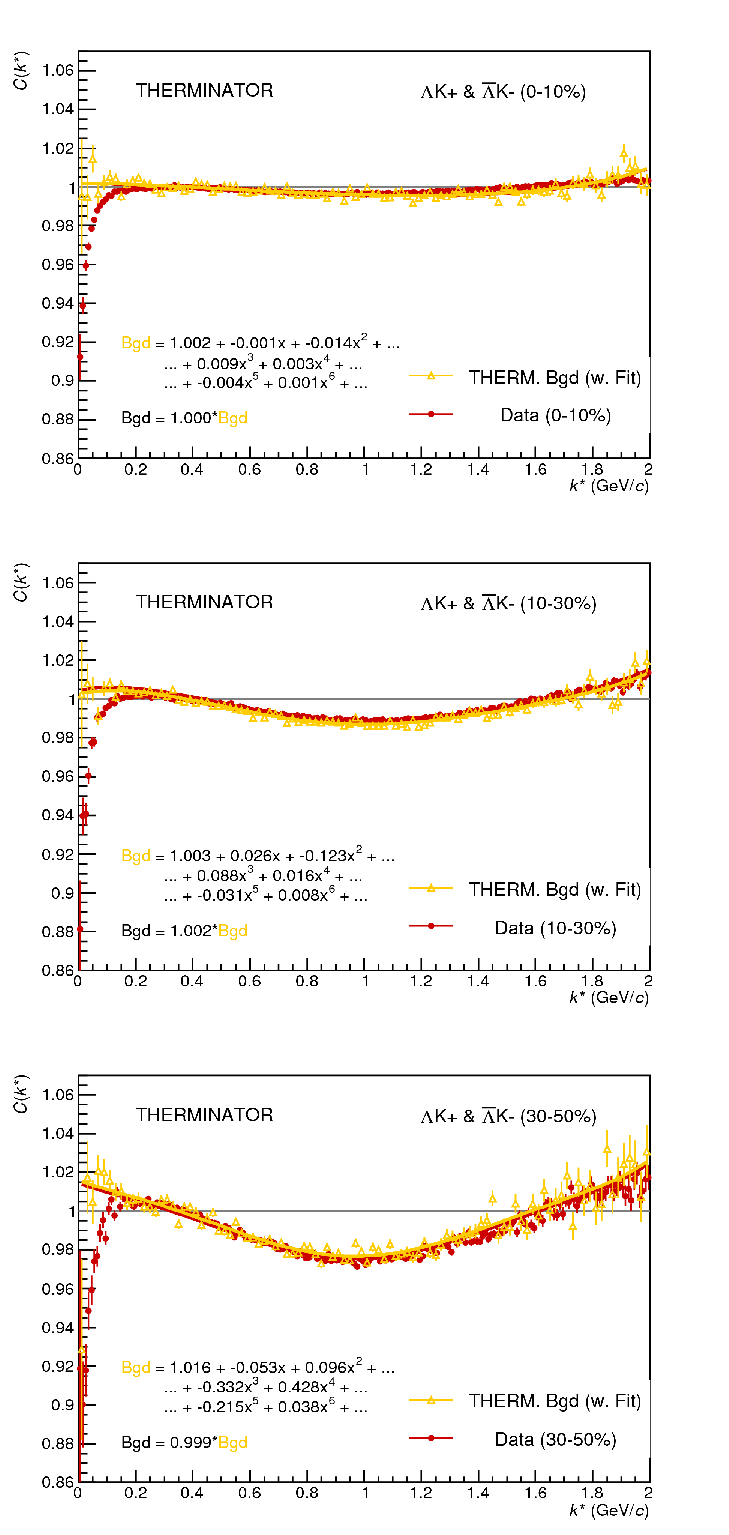
\includegraphics[width=0.30\textwidth]{/home/jesse/Analysis/FemtoAnalysis/AnalysisNotes/5_Fitting/Figures/BgdwFitOnly_RandomEPs_NumWeight1_PrimaryOnly_LamKchPwConj_0010_1030_3050.pdf}}
  %%----start of second subfigure---
  \subfigure[\LamKchM]{
    \label{fig:BgdswTHERM:b}
    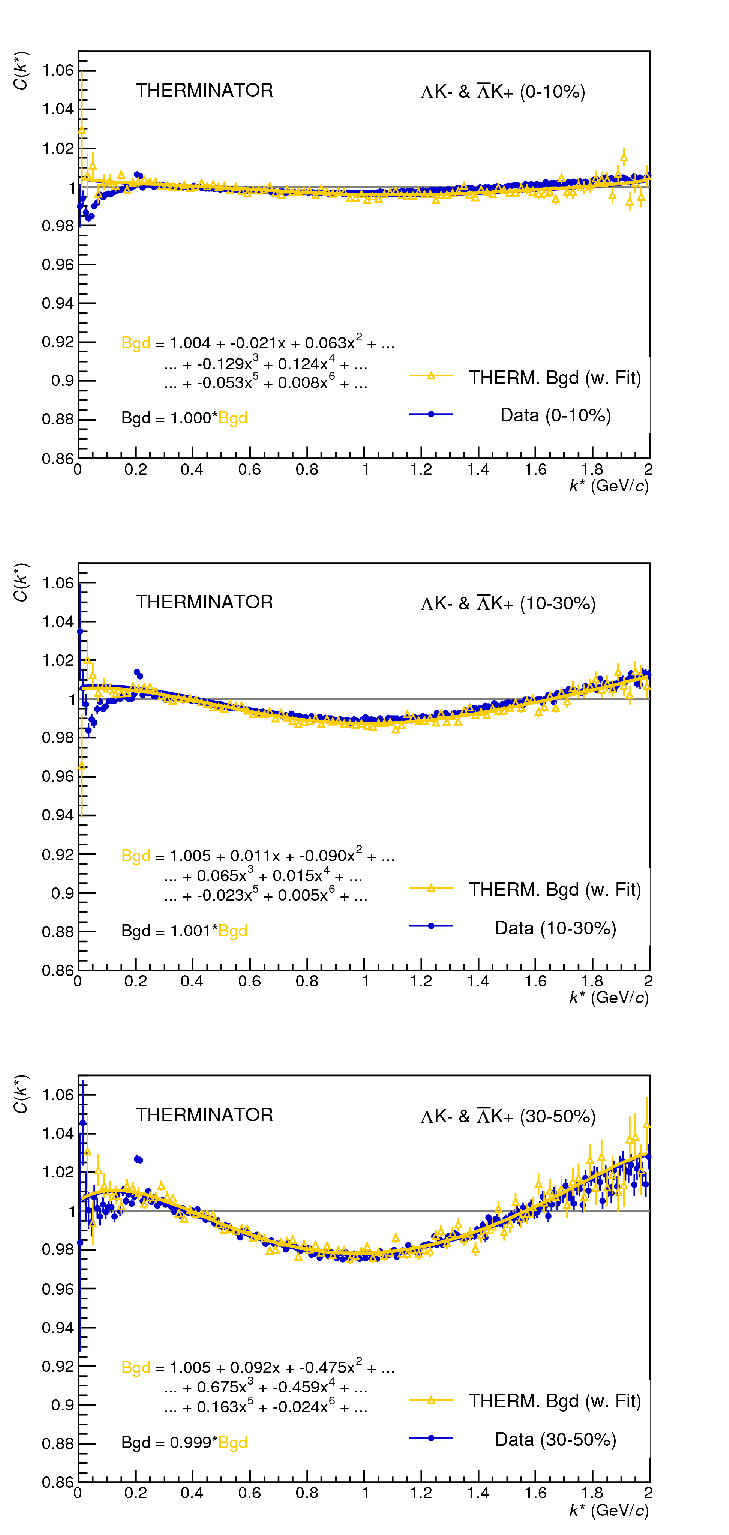
\includegraphics[width=0.30\textwidth]{/home/jesse/Analysis/FemtoAnalysis/AnalysisNotes/5_Fitting/Figures/BgdwFitOnly_RandomEPs_NumWeight1_PrimaryOnly_LamKchMwConj_0010_1030_3050.pdf}}
  %%----start of third subfigure---
  \subfigure[\LamKs]{
    \label{fig:BgdswTHERM:c}
    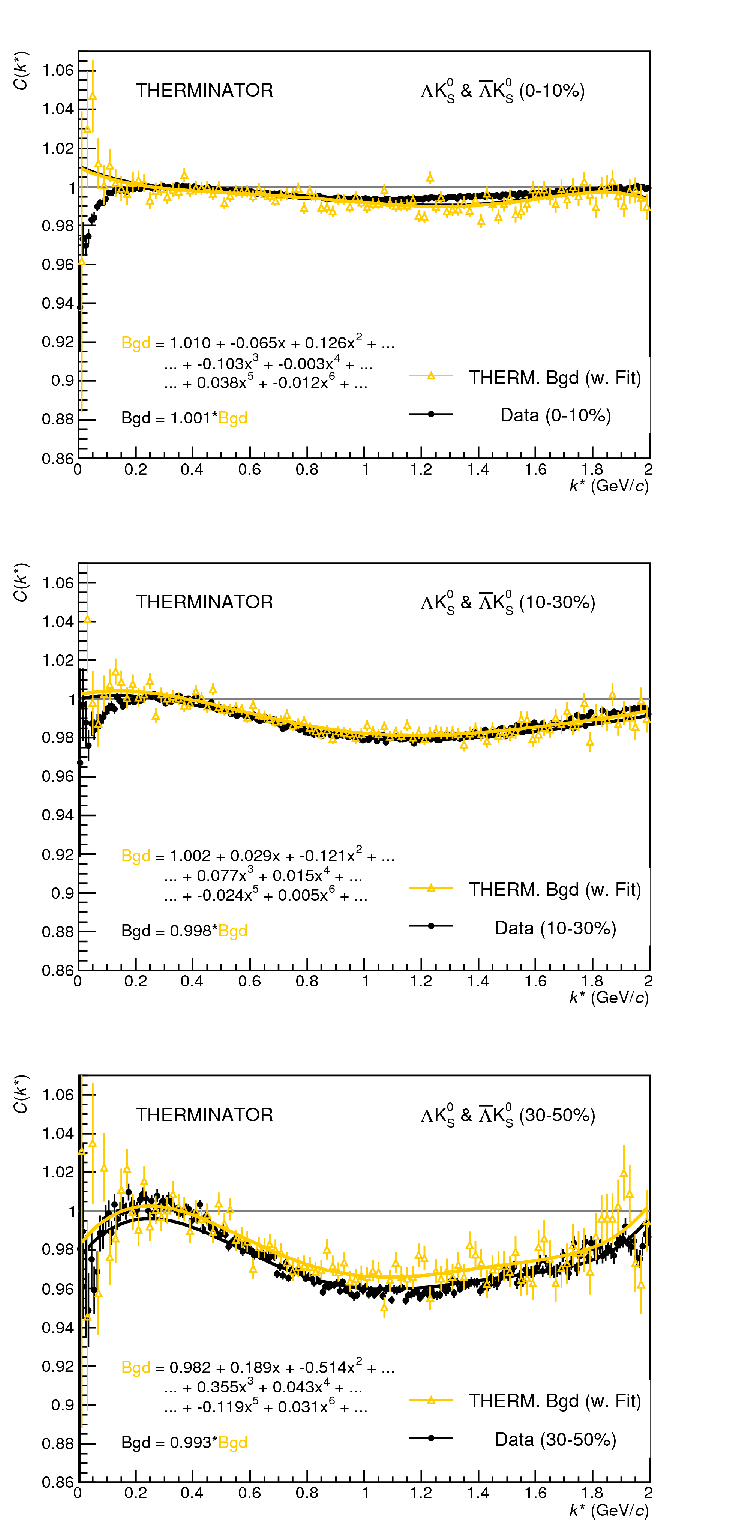
\includegraphics[width=0.30\textwidth]{/home/jesse/Analysis/FemtoAnalysis/AnalysisNotes/5_Fitting/Figures/BgdwFitOnly_RandomEPs_NumWeight1_PrimaryOnly_LamK0wConj_0010_1030_3050.pdf}}    
  %%----overall caption----
  \caption[Backgrounds with THERMINATOR]{THERMINATOR 2 simulation (gold) together with experimental data (red, blue, or black).  The left column shows results for \LamKchP (\ref{fig:BgdswTHERM:a}), middle for \LamKchM (\ref{fig:BgdswTHERM:b}), and right for \LamKs (\ref{fig:BgdswTHERM:c}).  A 6$^{th}$-order polynomial fit to the simulation is shown as a solid gold line, and whose fit parameters are printed on the lower left of each plot.  This polynomial is scaled to match the experimental data; the value of this scale is printed in the lower left corner of each plot.  The polynomial fit with scale factor applied is drawn in a color matching the experimental data (red, blue, black).}
  \label{fig:BgdswTHERM}
\end{figure}


An alternative approach to treating the non-femtoscopic background is to instead attempt to eliminate it.
The background may be effectively reduced by forming the reference distribution ($B(k^{*})$) with the ``Stavinskiy method".
With the Stavinskiy method, mixed-event pairs are not used for the reference distribution; instead, same-event pseudo-pairs, formed by rotating one particle in a real pair by 180$^\circ$ in the transverse plane, are used.  
This rotation rids the pairs of any femtoscopic correlation, while maintaining correlations due to elliptic flow (and other suitably symmetric contributors).
The effect on our \LamKchP correlation functions can be seen in the appendix, in Fig. \ref{fig:StavCfs_Correct_LamKchP}.


\subsection{Summarized Fit Procedure}
\label{SummarizedFitProcedure}


A simple $\chi^{2}$ test is inappropriate for fitting correlation functions, as the ratio two Poisson distributions does not result in a Poisson distribution.
Instead, a log-likelihood fit function of the following form is used \cite{Lisa:2005dd}:

\begin{equation}
 \chi^{2}_{PML} = -2\left[A\ln\left(\frac{C(A+B)}{A(C+1)}\right) + B\ln\left(\frac{A+B}{B(C+1)}\right)\right]
\label{eqn:Chi2PML}
\end{equation}

where $A$ is the experimental signal distribution (numerator), $B$ is the experimental reference distribution (denominator), and $C$ is the theoretical fit correlation function.
Therefore, we use Eq. \ref{eqn:Chi2PML} as the statistic quantifying the quality of the fit.
The parameters of the fit are: $\lambda$, $R$, $f_{0}$ ($\Re f_{0}$ and $\Im f_{0}$ separately), $d_{0}$, and normalization $N$.

With our procedure, we are able to share parameters between different analyses and fit all simultaneously.
A given pair and its conjugate (e.g. \LamKchP and \ALamKchM) always share scattering parameters ($\Re f_{0}$, $\Im f_{0}$, $d_{0}$).
However, the three distinct analyses (\LamKchP, \LamKchM, and \LamKs) are assumed to have scattering parameters unique from each other.
We assume the pair emission source for a given centrality class is similar between all analyses; therefore, for each centrality, all \LamK analyses share a common radius parameter.
We assume the same is true for the overall normalization $\lambda$ parameters in Eq. \ref{eqn:CfwRes}.
Finally, each correlation function has a unique normalization parameter.

All correlation functions were normalized in the range 0.32 $< k^{*} <$ 0.40 GeV/c, and fit in the range 0.0 $< k^{*} <$ 0.30 GeV/c.
For the \LamKchM analysis, the region 0.19 $< k^{*} <$ 0.23 GeV/$c$ was excluded from the fit to exclude the bump caused by the $\Omega^{-}$ resonance.
For each pair system, we account for contributions from three residual contributors, as discussed in Sec. \ref{ResidualCorrelations}, and whose individual $\lambda$ values are listed in Table \ref{tab:LambdaValues_All} (the cases of zero and ten residual contributors were also investigated, but the case of three contributors was deemed most reasonable).
We account for effects of finite track momentum resolution, as outlined in Sec. \ref{MomentumResolutionCorrections}.
The non-femtoscopic backgrounds are modeled using the THERMINATOR 2 simulation for the \LamKpm analyses, and with a linear form for the \LamKs system, as described in Sec. \ref{NonFlatBackground}.
In general, corrections are applied to the fit function, the raw data is never touched.

To summarize, the complete fit function is constructed as follows:
\begin{enumerate}
 \item The uncorrected, primary, correlation function, $C_{\Lambda\mathrm{K}}$(\ktrue), is constructed using Eqns. \ref{eqn:LednickyEqn} and \ref{eqn:CFSI}
 \item The correlation functions describing the parent systems which contribute residually are obtained using:
 \begin{itemize}
  \item Eqns. \ref{eqn:LednickyEqn} and \ref{eqn:CFSI} for the case of Coulomb-neutral pairs
  \item \XiKpm experimental data for \XiKpm contributions
  \item a Coulomb-only curve, with the help of Appendix \ref{App:CoulombFitter}, for other pairs including the Coulomb interaction 
 \end{itemize} 
 \item The residual contributions to the \LamK correlation function is found by running each parent correlation function through the appropriate transform matrix, via Eq.\ref{eqn:ResidualsTransform}
 \item The primary and residual correlations are combined, via Eq.\ref{eqn:Residuals} with Tab. \ref{tab:LambdaValues_All}, to form $C'_{Fit}$(\ktrue)
 \item The correlation function is corrected to account for momentum resolution effects using Eq. \ref{eqn:MomResCorrection}, to obtain $C'_{\mathrm{Fit}}(k^{*}_{\mathrm{Rec}})$
 \item Finally, the non-flat background correction, $F_{\mathrm{Bgd}}(k^{*}_{\mathrm{Rec}})$ is applied, and the final fit function is obtained, $C_{\mathrm{Fit}}(k^{*}_{\mathrm{Rec}}) = C'_{\mathrm{Fit}}(k^{*}_{\mathrm{Rec}})*F_{\mathrm{Bgd}}(k^{*}_{\mathrm{Rec}})$
\end{enumerate}

\subsection{Systematic uncertainties}
\label{SysErrs}

In order to understand the systematic uncertainties of our data, the analysis code was run many times using slightly different values for a number of important cuts, and the results were compared.  
To quantify the systematic errors on the data, all correlation functions built using all varied cut values were bin-by-bin averaged, and the resulting variance of each bin was taken as the systematic error.  
The cuts included in the systematic study, as well as the values used in the variations, are shown in Tab. \ref{tab:LamK0sSystematics} (\LamKs) and Tab. \ref{tab:LamKchSystematics} (\LamKpm).  
Note, the central value corresponds to that used in the analysis.

Similarly, the fit parameters extracted from all of these correlation functions were averaged, and the resulting variances were taken as the systematic errors for the fit parameters.
As with the systematic errors on the data, this was performed for all varied cut values.
Additionally, a systematic analysis was done on our fit method through varying our \kstar fit range, as well as varying our modeling of the non-femtoscopic background.
Our choice of \kstar fit range was varied by $\pm$ 25\%. 
As previously stated, the non-femtoscopic backgrounds are modeled using the THERMINATOR 2 simulation for the \LamKpm analyses, and with a linear form for the \LamKs system.
To study the contribution of this choice to our systematic errors, we modeled the backgrounds of all of our systems by fitting to the data with a with a linear, quadratic, and Gaussian form.
Additionally, we modeled the backgrounds of all systems with a polynomial fit to the THERMINATOR simulation, scaled to match the data. 
The resulting uncertainties in the extracted parameter sets were combined with our uncertainties arising from our particle and pair cuts.


\begin{table}[htbp]
 \centering 
  \renewcommand{\arraystretch}{1.2}
  \begin{tabular}{c|c}
   \multicolumn{2}{c}{\LamKs systematics} \\
   \hline  
   DCA \LamALam & 4, 5, 6 mm \\
   \hline
   DCA \Ks & 2, 3, 4 mm \\
   \hline
   DCA \LamALam Daughters & 3, 4, 5 mm \\
   \hline
   DCA \Ks Daughters & 2, 3, 4 mm \\
   \hline
   \LamALam Cosine of Pointing Angle & 0.9992, 0.9993, 0.9994 \\
   \hline
   \Ks Cosine of Pointing Angle & 0.9992, 0.9993, 0.9994 \\
   \hline
   DCA to Primary Vertex of p($\bar{\mathrm{p}}$) Daughter of \LamALam & 0.5, 1, 2 mm \\
   \hline
   DCA to Primary Vertex of $\pi^{-}$($\pi^{+}$) Daughter of \LamALam &  2, 3, 4 mm \\ 
   \hline
   DCA to Primary Vertex of $\pi^{+}$ Daughter of \Ks & 2, 3, 4 mm \\
   \hline
   DCA to Primary Vertex of $\pi^{-}$ Daughter of \Ks & 2, 3, 4 mm \\
   \hline
   Average Separation of Like-Charge Daughters & 5, 6, 7 cm \\
   \hline
  \end{tabular}
 \caption{\LamKs systematics}
 \label{tab:LamK0sSystematics} 
\end{table}


\begin{table}[htbp]
 \centering 
  \renewcommand{\arraystretch}{1.2}
  \begin{tabular}{c|c}
   \multicolumn{2}{c}{\LamKpm systematics} \\
   \hline  
   DCA \LamALam & 4, 5, 6 mm \\
   \hline
   DCA \LamALam Daughters & 3, 4, 5 mm \\
   \hline
   \LamALam Cosine of Pointing Angle & 0.9992, 0.9993, 0.9994 \\
   \hline
   DCA to Primary Vertex of p($\bar{\mathrm{p}}$) Daughter of \LamALam &  0.5, 1, 2 mm \\
   \hline
   DCA to Primary Vertex of $\pi^{-}$($\pi^{+}$) Daughter of \LamALam &  2, 3, 4 mm  \\
   \hline
   Average Separation of \LamALam Daughter with Same Charge as \Kpm & 7, 8, 9 cm \\
   \hline
   Max. DCA to Primary Vertex in Transverse Plane of \Kpm & 1.92, 2.4, 2.88 \\
   \hline
   Max. DCA to Primary Vertex in Longitudinal Direction of \Kpm & 2.4, 3.0, 3.6 \\
   \hline
  \end{tabular}
 \caption{\LamKpm systematics}
 \label{tab:LamKchSystematics} 
\end{table}



%\clearpage
\section{Results}
\label{sec:Results}

Figure \ref{fig:LamKFits_3Res} shows our \LamK data with fits for all studied centrality bins (0-10\%, 10-30\%, and 30-50\%). 
All analyses were fit simultaneously across all centralities, with a single radius and normalization $\lambda$ parameter for each centrality bin.
Scattering parameters ($\Re f_{0}$, $\Im f_{0}$, $d_{0}$) were shared between pair-conjugate systems, but assumed unique between the different \LamK charge combinations (i.e. a parameter set describing the \LamKchP \& \ALamKchM system, a second set describing the \LamKchM \& \ALamKchP system, and a third for the \LamKs \& \ALamKs system).
Each correlation function received a unique normalization parameter.
The fits were corrected for finite momentum resolution effects, non-femtoscopic backgrounds, and residual correlations resulting from the feed-down from resonances.
In Fig. \ref{fig:LamKFits_3Res}, lines represent statistical errors, while boxes represent systematic errors.  The black solid curve shows the primary (\LamK) contribution to the fit, the green curve shows the fit to the non-femtoscopic background, and the purple curve shows the final fit after all corrections have been applied.
The extracted fit values with uncertainties are printed as (fit value) $\pm$ (statistical uncertainty) $\pm$ (systematic uncertainty).

\begin{figure}[htp]
  \centering
  %%----start of first subfigure---
  \subfigure[\LamKchPALamKchM]{
    \label{fig:LamKFits_3Res:a}
    \includegraphics[width=0.49\linewidth]{\ResultsDirBaseLamKch\SaveNameModLamKch/canKStarCfwFitsLamKchPwConj_0010_1030_3050\SaveNameModLamKch.pdf}}
  %%----start of second subfigure---  
  \subfigure[\LamKchMALamKchP]{
    \label{fig:LamKFits_3Res:b}
    \includegraphics[width=0.49\linewidth]{\ResultsDirBaseLamKch\SaveNameModLamKch/canKStarCfwFitsLamKchMwConj_0010_1030_3050\SaveNameModLamKch.pdf}}
  \\  
  %%----start of third subfigure---  
  \subfigure[\LamKsALamKs]{
    \label{fig:LamKFits_3Res:c}
    \includegraphics[width=0.49\linewidth]{\ResultsDirBaseLamKs\SaveNameModLamKs/canKStarCfwFitsLamK0wConj_0010_1030_3050\SaveNameModLamKs.pdf}}    
  %%----overall caption----
  \caption{Fits, with 3 residual correlations included, for all \LamK analyses across all studied centralities (0-10\%, 10-30\%, and 30-50\%).
 The lines represent the statistical errors, while the boxes represent the systematic errors.
 The black solid line represents the primary (\LamK) correlation's contribution to the fit.  
 The green line shows the fit to the non-flat background.
 The purple points show the fit after all residuals' contributions have been included, and momentum resolution and non-flat background corrections have been applied.
 The extracted fit values with uncertainties are printed.}  
  \label{fig:LamKFits_3Res}
\end{figure}

\begin{figure}[h]
  \centering
  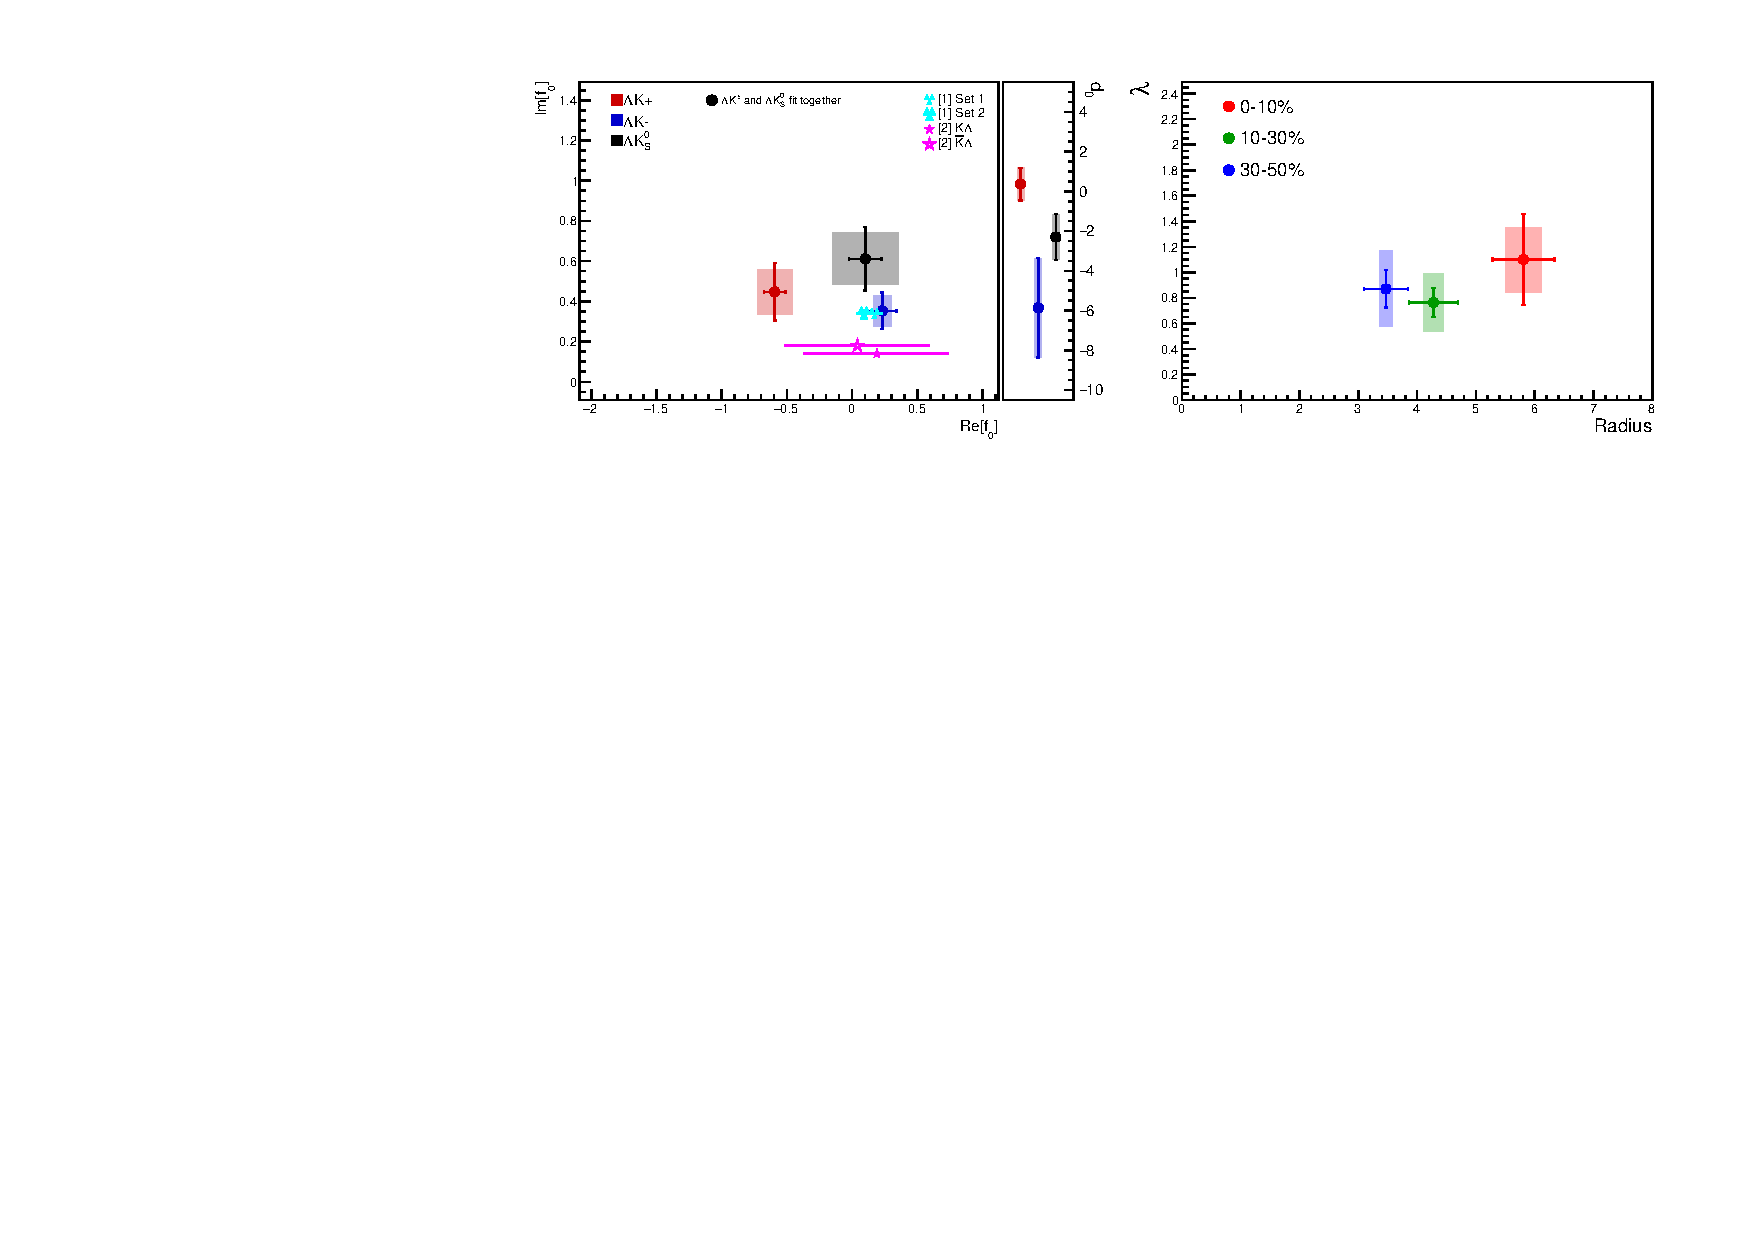
\includegraphics[width=\textwidth]{./Comp3An_Triple.pdf}
  \caption[Extracted Scattering Parameters]{Extracted scattering parameters for all of our $\Lambda$K systems.  [Left]: $\Im f_{0}$ vs. $\Re f_{0}$, together with $d_{0}$ to the right.  [Right]: $\lambda$ vs. Radius for the studied centrality bins (0-10\%, 10-30\%, 30-50\%).  The green \cite{Liu:2006xja} and yellow \cite{Mai:2009ce} points show theoretical predictions made using chiral perturbation theory.}
  \label{fig:ScattParams_3Res}
\end{figure}

Figure \ref{fig:ScattParams_3Res} summarizes well our results.
In the summary plot, we show the extracted scattering parameters in the form of a $\Im f_{0}$ vs $\Re f_{0}$ plot, which includes the $d_{0}$ values to the right side.  
We also show the $\lambda$ vs. radius parameters for all three of our studied centrality bins. 
In addition to our results, we show theoretical predictions made using chiral perturbation theory \cite{Liu:2006xja,Mai:2009ce}.

We extract positive imaginary parts, $\Im(f_{0})$, of the scattering lengths for all systems. 
We expect this, as $\Im(f_{0})$ describes the inelastic scattering channels.
More interestingly, our results show that the \LamKchP and \LamKchM systems differ in the sign of the real part, $\Re(f_{0})$, of their scattering lengths (negative for \LamKchP, and positive for \LamKchM).
Furthermore, each of the three systems has a $\Re(f_{0})$ unique from the others.
The real part of the scattering length describes the effect of the strong interaction, making the difference in these systems quite intriguing.
A positive $\Re(f_{0})$ signifies that the effect of the strong force is attractive, which a negative $\Re(f_{0})$ signifies a repulsion.
We suggest that this difference could be due to an effect arising from different quark-antiquark interactions between the pairs ($\rm s\bar{s}$ in \LamKchP, $\rm u\bar{u}$ in \LamKchM).
An alternative explanation could be that the effect is due to the different net strangeness for each system.
More specifically, systems with less net strangeness have more channels into which they can decay, causing a scarcity of pairs, i.e. a greater suppression of the correlation function, at low-\kstar.
However, an effect such as this really should instead manifest itself in $\Im(f_{0})$ not $\Re(f_{0})$.
In any case, this remains a very interesting effect which needs an explanation.

\begin{figure}[h]
  \centering
  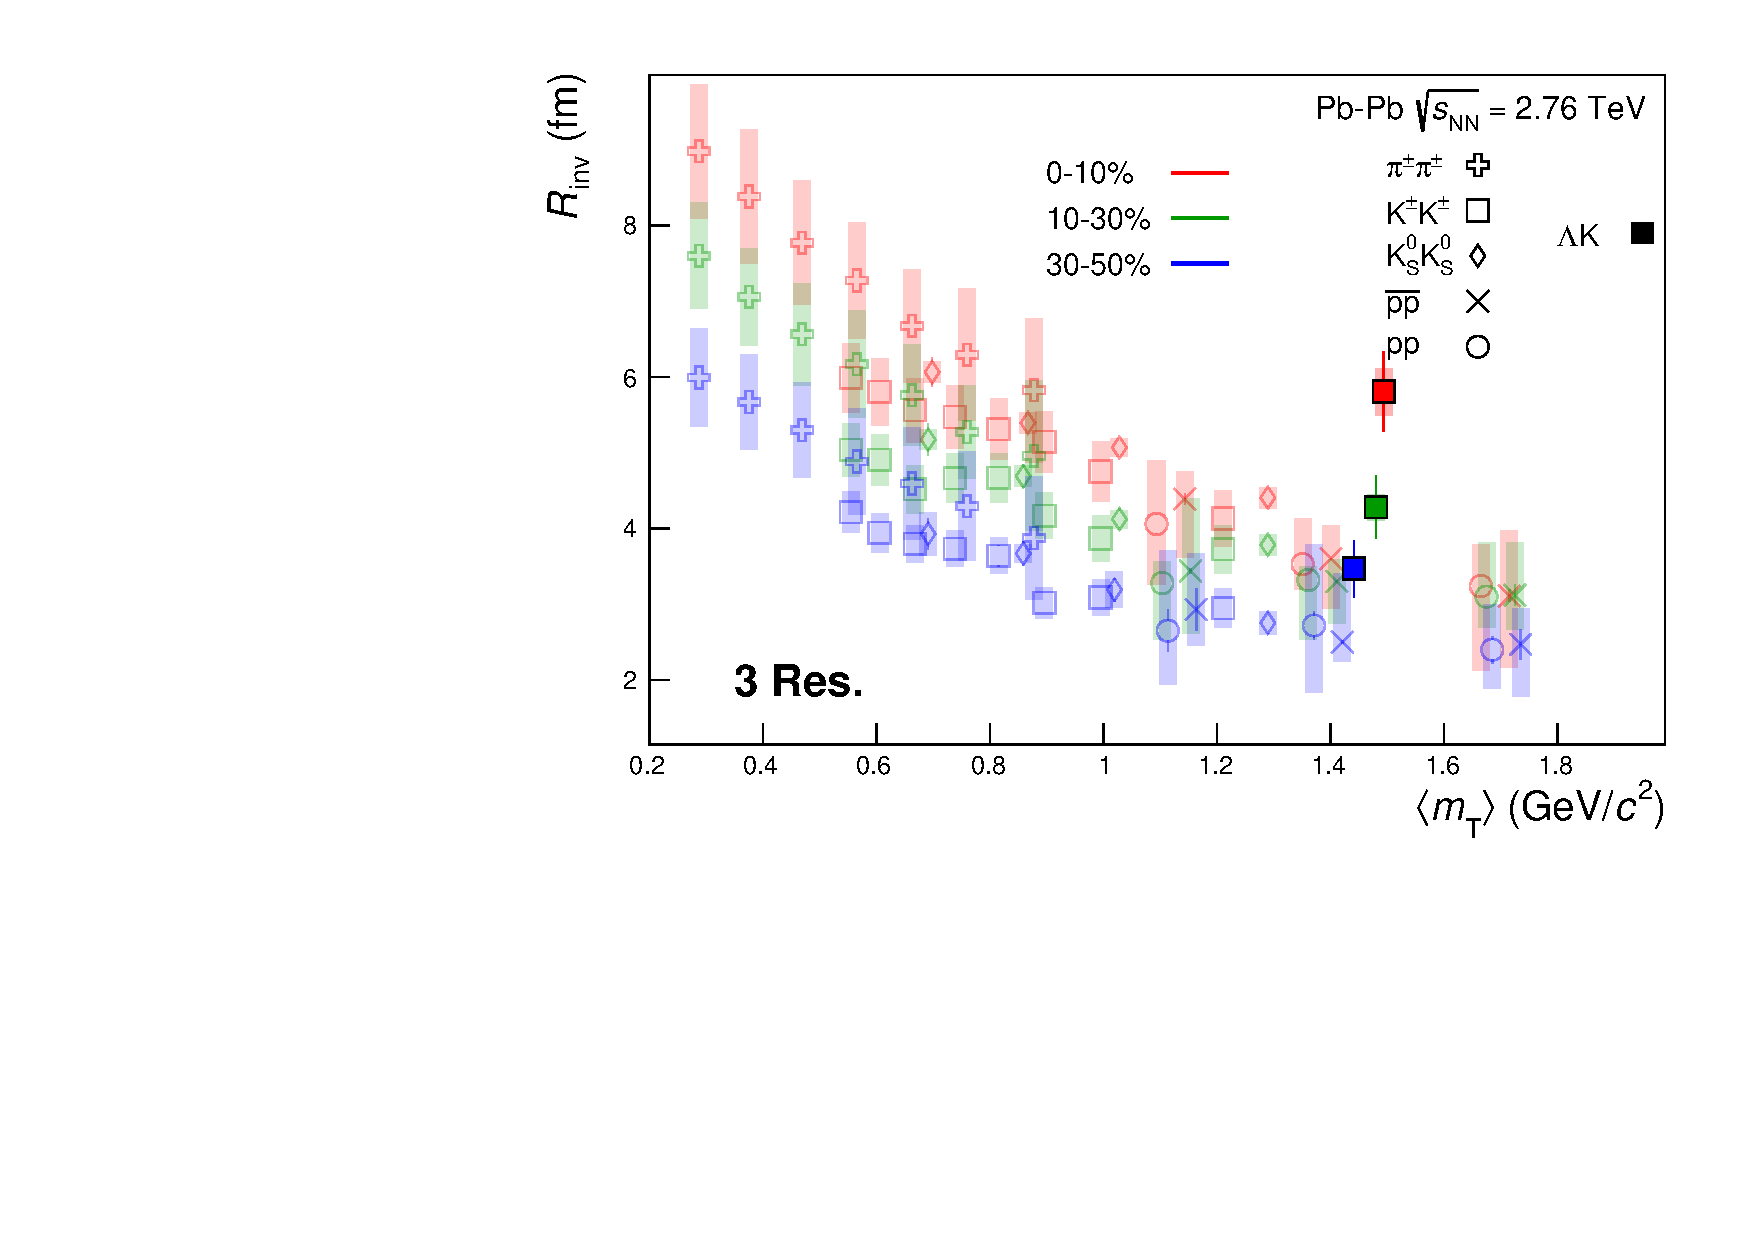
\includegraphics[width=0.75\textwidth]{./mTscaling.pdf}
  \caption[\mt Scaling of Radii: 3 Residuals in Fit]{3 residual correlations in \LamK fits.  Extracted fit $R_{\mathrm{inv}}$ parameters as a function of pair transverse mass (\mt) for various pair systems over several centralities. The ALICE published data \cite{Adam:2015vja} is shown with transparent, open symbols.}
  \label{fig:mTScalingOfRadii_3Res}
\end{figure}

A comparison of our extracted radii to those of other systems measure by ALICE \cite{Adam:2015vja} is shown in Figure \ref{fig:mTScalingOfRadii_3Res}. 
The figure shows extracted $R_{\mathrm{inv}}$ vs. \mt for several centralities and for several different systems.
The radii are observed to increase for more central events, as expected from a simple geometric picture of the collisions.
They also demonstrate a decreasing size with increasing \mt, as expected in the presence of collective radial flow \cite{Akkelin:1995gh}.
It was found that \cite{Kisiel:2014upa}, even in the presence of good global \mt-scaling for the three-dimensional radii in the LCMS frame, a particle species dependence will exist for the $R_{\mathrm{inv}}$ measured in the PRF, due to trivial kinematic reasons.
These kinematic effects, resulting from the transformation from LCMS to PRF, causes smaller masses to exhibit larger $R_{\mathrm{inv}}$ \cite{Adam:2015vja} (explaining, for instance, how the pion radii are systematically higher than kaon radii at the same approximate \mt).



It is clear from the results that the \LamK systems do not conform to the approximate \mt-scaling of the pair source sizes.\footnote[1]
{
For our non-identical particle pairs, to be more directly analogous to the single particle \mt, we define the pair transverse mass as

\begin{equation*}
\begin{aligned}
 m_{\mathrm{T, pair}}^{2} &= \left( \frac{m_{\mathrm{inv}}}{2} \right)^{2} + \left( \frac{1}{2} |\textbf{\textit{p}}_{\mathrm{T,1}} + \textbf{\textit{p}}_{\mathrm{T,2}}| \right)^{2} \\
 &= (K^{0})^{2} - (K^{3})^{2} \\
 &\mathrm{where} ~~K^{\mu} \equiv \frac{1}{2} \left( p_{1}^{\mu} + p_{2}^{\mu} \right)
\end{aligned}
\label{eqn:PairmTv1}
\end{equation*}
}
At first thought, this may appear to be a troubling result; the approximate scaling is an observed consequence of the collective behavior of the soft (low-\pt) sector of the produced system.
The \Lam and K particles certainly participate in the collective expansion of the QGP medium, but, importantly, they are non-identical particles.
Taking a closer look at Fig. \ref{fig:mTScalingOfRadii_3Res}, one can see that the previously published data (transparent points), and the established (approximate) \mt-scaling trend, are for identical particle analyses only.
When dealing with non-identical particles, the pair emission source, which is measured by femtoscopy, is the superposition of two single-particle sources.
In general, each single-particle source will have its own size, shape, and space-time position within the produced medium, which is unique from its paired partner.
The hydrodynamic nature of the medium produces the approximate \mt-scaling with respect to these single-particle sources, not the pair sources.
The combination of two unique sources separated in space-time, when probing correlations between non-identical particle pairs, leads to extracted radii falling outside of the (identical particle femtoscopy) \mt-scaling trend.

It is well established that non-identical particle femtoscopic studies are able to probe deeper than the second moments of the pair distribution functions accessed via identical particle studies.
In addition to this, non-identical particle studies are able to measure the relative emission shifts, the first moments of the emission function.
For the study of \LamK pairs at mid-rapidity in Pb-Pb collisions, we expect a separation of the single-particle sources in the out direction.
One elegant method for extracting information about the emission asymmetries is via a spherical decomposition of the correlation function.
With this method, one can draw a wealth of information from just a few components of the decomposition.
Particularly, the $C_{00}$ component is similar to the 1D correlation functions typically studied, and probes the overall size of the source.
The $\Re C_{11}$ component probes the asymmetry of the system in the out direction; a non-zero value reveals the asymmetry. 
Figure \ref{fig:LamKchP_ReC00C11_0010} in App. \ref{app:SphericalHarmonics} shows the $C_{00}$ and $\Re C_{11}$ components of the spherical decomposition of our \LamKchP data in the 0-10\% centrality bin.
The $\Re C_{11}$ component shows a clear deviation from zero, and the negative value signifies that the \Lam particles are, on average, emitted further out and/or earlier than the K mesons.
This effect is supported by the results obtained from the THERMINATOR 2 model, shown in Fig. \ref{fig:LamKchP_StdThermSources}.
The effect of a non-zero shift in the source will naturally lead to larger measured radii.
This is intuitive, and also reaffirmed in our simulation with THERMINATOR 2 shown in App. \ref{app:THERM}.
We have also shown larger effective radii to result from inserting a Gaussian source with a non-zero shift into the Koonin-Pratt equation and numerically integrating.

\section{Summary}
\label{sec:Summary}

Results from a femtoscopic analysis of \LamK correlations in Pb-Pb collisions at $\sqrt{s_{\mathrm{NN}}}$ = 2.76 TeV with ALICE at the LHC have been presented.
The femtoscopic radii, $\lambda$ parameters, and scattering parameters were extracted from one-dimensional correlation functions in terms of the invariant momentum difference.
The scattering parameters of \LamK pairs in all three charge combinations (\LamKchP, \LamKchM, and \LamKs) have been measured for the first time.
We observe a striking difference in the \LamKchP and \LamKchM correlation functions, which is reflected in the unique set of scattering parameters extracted for each.
The \LamKchP systems exhibits a negative $\Re(f_{0})$, while that extracted from the \LamKchM system is positive.
The physics underlying this phenomenon is currently not well understood, but we suggest this could be due to different quark-antiquark interactions between the pairs, or from different net strangeness for each system. 
Finally, we find that the \LamK systems exhibit source radii larger than expected from extrapolation from identical particle femtoscopic studies.
We understand this effect to result from the separation in space-time of the single-particle \Lam and K source distributions.


%\clearpage

%%%%% acknowledgements
\newenvironment{acknowledgement}{\relax}{\relax}
\begin{acknowledgement}
\section*{Acknowledgements}
%\input{acknowledgements.tex}    %%%%%%% done by webmaster team
\end{acknowledgement}

%%%%%%%% Bibliography (In case of using bibtex generate the bbl requested by arXiv)
\bibliographystyle{utphys}   % Remember we use title in the biblio
\bibliography{LamK_bibfile}
%\input {bibliography.tex}  

%%%%%%%%% appendix with author list
\newpage
\appendix
%
%% Following lines needed so, for instance, Fig D.1(a) not printed as simply 1(a) when referenced
\renewcommand{\thesubfigure}{\thefigure(\alph{subfigure})}
\makeatletter
\renewcommand{\p@subfigure}{}
\renewcommand{\@thesubfigure}{(\alph{subfigure})\hskip\subfiglabelskip}
%\input{}               %%%%%%%%%%% put your appendices here
%


\pagestyle{empty}
\begin{landscape}

\section{$\lambda$ Parameters}
\label{App:LamParams}

\begin{table}[htbp]
 \centering
 \renewcommand{\arraystretch}{1.2}
 \resizebox{\paperwidth}{!}{
 \begin{tabular}{|c|cV{5.0}c|cV{5.0}c|cV{5.0}c|cV{5.0}c|cV{5.0}c|c|}
  \multicolumn{2}{c}{\LamKchP residuals} & \multicolumn{2}{c}{\ALamKchM residuals} & \multicolumn{2}{c}{\LamKchM residuals} & \multicolumn{2}{c}{\ALamKchP residuals} & \multicolumn{2}{c}{\LamKs residuals} & \multicolumn{2}{c}{\ALamKs residuals} \\
  \hline
  \textbf{Pair System} & \textbf{$\lambda$ value} & \textbf{Pair System} & \textbf{$\lambda$ value} & \textbf{Pair System} & \textbf{$\lambda$ value} & \textbf{Pair System} & \textbf{$\lambda$ value} & \textbf{Pair System} & \textbf{$\lambda$ value} & \textbf{Pair System} & \textbf{$\lambda$ value} \\
  \hlineB{3.0}
  \multicolumn{12}{|c|}{3 Residuals (Max Parent $c\tau_{\mathrm{decay}}$ = 10 fm)} \\
  \hlineB{3.0}
  $\Lambda$K$^{+}$ & 0.527 & $\bar{\Lambda}$K$^{-}$ & 0.526 & $\Lambda$K$^{-}$ & 0.526 & $\bar{\Lambda}$K$^{+}$ & 0.527 & $\Lambda$K$^{0}_{\mathrm{S}}$ & 0.543 & $\bar{\Lambda}$K$^{0}_{\mathrm{S}}$ & 0.544 \\
  
  $\Sigma^{0}$K$^{+}$ & 0.111 & $\bar{\Sigma}^{0}$K$^{-}$ & 0.110 & $\Sigma^{0}$K$^{-}$ & 0.110 & $\bar{\Sigma}^{0}$K$^{+}$ & 0.111 & $\Sigma^{0}$K$^{0}_{\mathrm{S}}$ & 0.120 & $\bar{\Sigma}^{0}$K$^{0}_{\mathrm{S}}$ & 0.120 \\
  
  $\Xi^{0}$K$^{+}$ & 0.039 & $\bar{\Xi}^{0}$K$^{-}$ & 0.035 & $\Xi^{0}$K$^{-}$ & 0.038 & $\bar{\Xi}^{0}$K$^{+}$ & 0.036 & $\Xi^{0}$K$^{0}_{\mathrm{S}}$ & 0.042 & $\bar{\Xi}^{0}$K$^{0}_{\mathrm{S}}$ & 0.039 \\
  
  $\Xi^{-}$K$^{+}$ & 0.050 & $\bar{\Xi}^{+}$K$^{-}$ & 0.046 & $\Xi^{-}$K$^{-}$ & 0.050 & $\bar{\Xi}^{+}$K$^{+}$ & 0.046 & $\Xi^{-}$K$^{0}_{\mathrm{S}}$ & 0.054 & $\bar{\Xi}^{+}$K$^{0}_{\mathrm{S}}$ & 0.050 \\
  
  Other & 0.226 & Other & 0.235 & Other & 0.228 & Other & 0.233 & Other & 0.194 & Other & 0.199 \\
  
  Fakes & 0.048 & Fakes & 0.048 & Fakes & 0.048 & Fakes & 0.048 & Fakes & 0.048 & Fakes & 0.048 \\
  
  \hlineB{3.0}  
  \multicolumn{12}{|c|}{10 Residuals (Max Parent $c\tau_{\mathrm{decay}}$ = 4 fm)} \\
  \hlineB{3.0}
  $\Lambda$K$^{+}$ & 0.180 & $\bar{\Lambda}$K$^{-}$ & 0.180 & $\Lambda$K$^{-}$ & 0.179 & $\bar{\Lambda}$K$^{+}$ & 0.181 & $\Lambda$K$^{0}_{\mathrm{S}}$ & 0.192 & $\bar{\Lambda}$K$^{0}_{\mathrm{S}}$ & 0.193 \\
  
  $\Sigma^{0}$K$^{+}$ & 0.116 & $\bar{\Sigma}^{0}$K$^{-}$ & 0.114 & $\Sigma^{0}$K$^{-}$ & 0.115 & $\bar{\Sigma}^{0}$K$^{+}$ & 0.116 & $\Sigma^{0}$K$^{0}_{\mathrm{S}}$ & 0.125 & $\bar{\Sigma}^{0}$K$^{0}_{\mathrm{S}}$ & 0.124 \\
  
  $\Xi^{0}$K$^{+}$ & 0.040 & $\bar{\Xi}^{0}$K$^{-}$ & 0.037 & $\Xi^{0}$K$^{-}$ & 0.040 & $\bar{\Xi}^{0}$K$^{+}$ & 0.037 & $\Xi^{0}$K$^{0}_{\mathrm{S}}$ & 0.043 & $\bar{\Xi}^{0}$K$^{0}_{\mathrm{S}}$ & 0.040 \\
  
  $\Xi^{-}$K$^{+}$ & 0.052 & $\bar{\Xi}^{+}$K$^{-}$ & 0.047 & $\Xi^{-}$K$^{-}$ & 0.052 & $\bar{\Xi}^{+}$K$^{+}$ & 0.048 & $\Xi^{-}$K$^{0}_{\mathrm{S}}$ & 0.056 & $\bar{\Xi}^{+}$K$^{0}_{\mathrm{S}}$ & 0.052 \\
  
  $\Sigma^{*+}$K$^{+}$ & 0.054 & $\bar{\Sigma}^{*-}$K$^{-}$ & 0.051 & $\Sigma^{*+}$K$^{-}$ & 0.053 & $\bar{\Sigma}^{*-}$K$^{+}$ & 0.051 & $\Sigma^{*+}$K$^{0}_{\mathrm{S}}$ & 0.058 & $\bar{\Sigma}^{*-}$K$^{0}_{\mathrm{S}}$ & 0.055 \\
  
  $\Sigma^{*-}$K$^{+}$ & 0.048 & $\bar{\Sigma}^{*+}$K$^{-}$ & 0.050 & $\Sigma^{*-}$K$^{-}$ & 0.048 & $\bar{\Sigma}^{*+}$K$^{+}$ & 0.050 & $\Sigma^{*-}$K$^{0}_{\mathrm{S}}$ & 0.052 & $\bar{\Sigma}^{*+}$K$^{0}_{\mathrm{S}}$ & 0.054 \\
  
  $\Sigma^{*0}$K$^{+}$ & 0.048 & $\bar{\Sigma}^{*0}$K$^{-}$ & 0.045 & $\Sigma^{*0}$K$^{-}$ & 0.048 & $\bar{\Sigma}^{*0}$K$^{+}$ & 0.045 & $\Sigma^{*0}$K$^{0}_{\mathrm{S}}$ & 0.052 & $\bar{\Sigma}^{*0}$K$^{0}_{\mathrm{S}}$ & 0.048 \\
  
  $\Lambda$K$^{*0}$ & 0.046 & $\bar{\Lambda}\bar{\mathrm{K}}^{*0}$ & 0.047 & $\Lambda\bar{\mathrm{K}}^{*0}$ & 0.046 & $\bar{\Lambda}$K$^{*0}$ & 0.047 & $\Lambda$K$^{*0}$ & 0.022 & $\bar{\Lambda}$K$^{*0}$ & 0.022 \\
  
  $\Sigma^{0}$K$^{*0}$ & 0.041 & $\bar{\Sigma}^{0}\bar{\mathrm{K}}^{*0}$ & 0.041 & $\Sigma^{0}\bar{\mathrm{K}}^{*0}$ & 0.041 & $\bar{\Sigma}^{0}$K$^{*0}$ & 0.041 & $\Sigma^{0}$K$^{*0}$ & 0.019 & $\bar{\Sigma}^{0}$K$^{*0}$ & 0.019 \\
  
  $\Xi^{0}$K$^{*0}$ & 0.014 & $\bar{\Xi}^{0}\bar{\mathrm{K}}^{*0}$ & 0.013 & $\Xi^{0}\bar{\mathrm{K}}^{*0}$ & 0.014 & $\bar{\Xi}^{0}$K$^{*0}$ & 0.013 & $\Xi^{0}$K$^{*0}$ & 0.007 & $\bar{\Xi}^{0}$K$^{*0}$ & 0.006 \\
  
  $\Xi^{-}$K$^{*0}$ & 0.018 & $\bar{\Xi}^{+}\bar{\mathrm{K}}^{*0}$ & 0.017 & $\Xi^{-}\bar{\mathrm{K}}^{*0}$ & 0.018 & $\bar{\Xi}^{+}$K$^{*0}$ & 0.017 & $\Xi^{-}$K$^{*0}$ & 0.009 & $\bar{\Xi}^{+}$K$^{*0}$ & 0.008 \\
  
  Other & 0.295 & Other & 0.310 & Other & 0.299 & Other & 0.307 & Other & 0.318 & Other & 0.330 \\
  
  Fakes & 0.048 & Fakes & 0.048 & Fakes & 0.048 & Fakes & 0.048 & Fakes & 0.048 & Fakes & 0.048 \\
  
  \hlineB{3.0}
 \end{tabular}}
 \caption{$\lambda$ values for the individual components of the \LamK correlation functions for the case of 3 and 10 residual contributions.}
 \label{tab:LambdaValues_All}
\end{table}

\end{landscape}
\pagestyle{plain}



\section{Stavinskiy Reference Method}
\label{App:StavMethod}

Another option for obtaining the reference distribution, $B(k^{*})$, is to use, what we will refer to as, the ``Stavinskiy method" \cite{Stavinskiy04}.
The method was first proposed to handle the case of one event femtoscopy, and has been suggested for use in eliminating momentum conservation effects in the reference distribution \cite{Lisa:2005dd}.
The method is appropriate for collisions between symmetric projectiles, at sufficiently large energy, with a detector which is symmetrical with respect to the transition $\mathbf{r} \rightarrow \mathbf{-r}$.
The purpose of our use of the Stavinskiy method is to rid the correlation functions of the non-femtoscopic background.  
More specifically, our intent is to handle background contributions from elliptic flow, and other sources having reflection symmetry in the transverse plane.  
With the Stavinskiy method, mixed-event pairs are not used for the reference distribution; instead, same-event pseudo-pairs, formed by rotating one particle in a real pair by 180$^\circ$ in the transverse plane, are used.  
This rotation rids the pairs of any femtoscopic correlation, while maintaining correlations due to elliptic flow (and other suitably symmetric contributors).

The results of correctly implementing such a procedure are shown in Figure \ref{fig:StavCfs_Correct_LamKchP}.  
The figure shows the Stavinskiy method does a very good job of ridding the \LamKpm correlations of their non-femtoscopic backgrounds.  
We also see the procedure does not work as well on the \LamKs system.


\begin{figure}[h!]
  \centering
  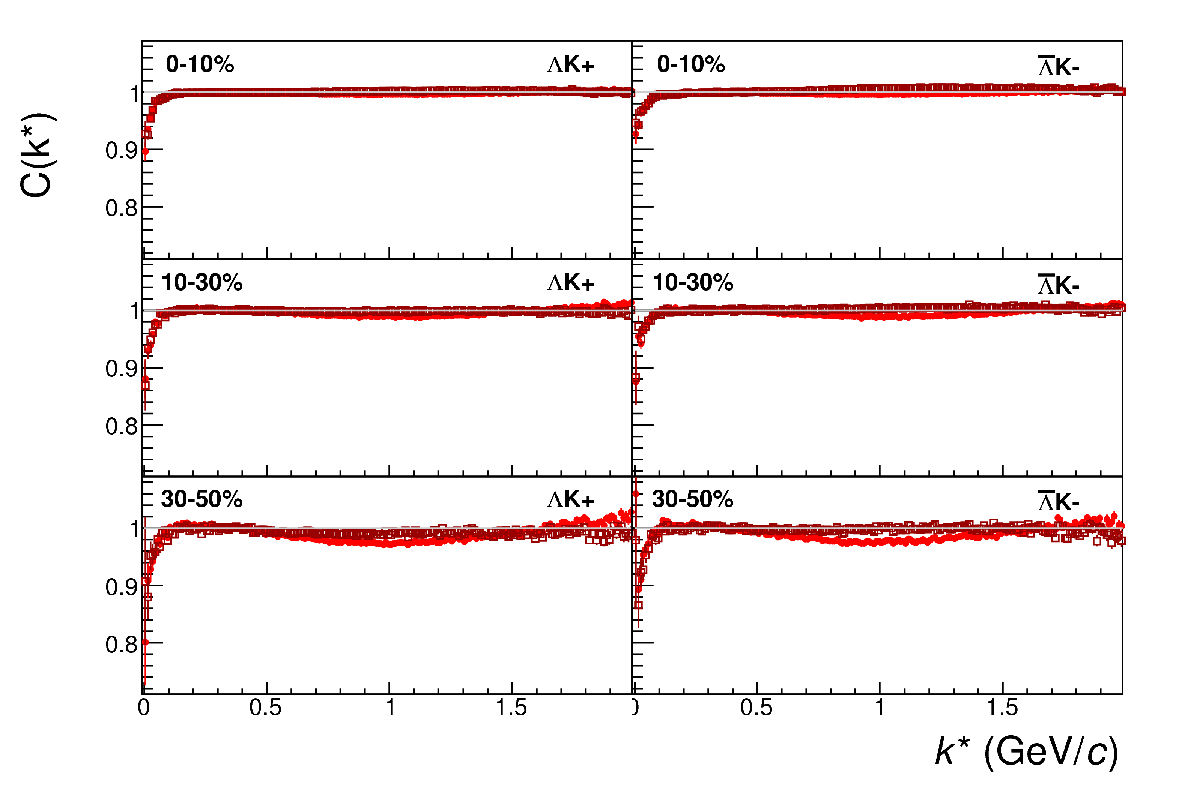
\includegraphics[width=\textwidth]{/home/jesse/Analysis/FemtoAnalysis/AnalysisNotes/4_CorrelationFunctions/Figures/WithAdditionalPairCut_20180505/canKStarCfsLamKchPwConj_20180505vs20180505StavCf.pdf}
  \caption[\LamKchP Stavinskiy Correlation Functions]{\LamKchPALamKchM correlation functions built using the Stavinskiy method for 0-10\%, 10-30\%, and 30-50\% centralities.  Closed symbols represent correlations built using the normal mixed-event reference distribution, while open symbols represent correlations formed using the Stavinskiy same-event pseudo-pairs as a reference.}
  \label{fig:StavCfs_Correct_LamKchP}
\end{figure}

Now, one must be somewhat careful when applying this Stavinskiy method.  
We found that, in order to obtain correct results, we had to run our pseudo-pairs through the same pair cuts used in our analyses.  
In an ideal world, our pair cut would only remove truly bad pairs results from splitting, merging, etc.  
In the real world, the pair cut always throws out some of the good with the bad.  
For the pseudo-pairs to form a reliable reference, they too must experience the pair cut, and the loss of ``good'' pseudo-pairs.  
We found this issue affected mainly our \LamKchP \& \ALamKchM analysis.



\section{Strong and Coulomb Fitter}
\label{App:CoulombFitter}

When modeling systems which include both strong and Coulomb effects, Eq. \ref{eqn:LednickyEqn} is no longer valid, and, in fact, there is no analytical form with which to fit.
To solve such a problem, and to fit such a system, one must develop a more fundamental model, beginning with Eq. \ref{eqn:KooninPrattEqn} and using the two-particle wave-function including both strong and Coulomb interactions \cite{Lednicky:2005tb}:

\begin{equation}
 \Psi_{\mathbf{k^{*}}}(\mathbf{r^{*}}) = e^{i\delta_{c}}\sqrt{A_{c}(\eta)}[e^{i\mathbf{k^{*}} \cdot \mathbf{r^{*}}}F(-i\eta,1,i\xi) + f_{c}(k^{*})\frac{\tilde{G}(\rho,\eta)}{r^{*}}]
\label{eqn:CoulombWaveFcn}
\end{equation}

where $\rho = k^{*}r^{*}$, $\eta = (k^{*}a_{c})^{-1}$, $\xi = \mathbf{k^{*}} \cdot \mathbf{r^{*}} + k^{*}r^{*} \equiv \rho(1+\cos\theta^{*})$, and $a_{c} = (\mu z_{1}z_{2}e^{2})^{-1}$ is the two-particle Bohr radius (including the sign of the interaction).  
$\delta_{c}$ is the Coulomb s-wave phase shift, $A_{c}(\eta)$ is the Coulomb penetration factor, $\tilde{G} = \sqrt{A_{c}}(G_{0} + iF_{0})$ is a combination of the regular ($F_{0}$) and singular ($G_{0}$) s-wave Coulomb functions.  
$f_{c}(k^{*})$ is the s-wave scattering amplitude:

\begin{equation}
 f_{c}(k^{*}) = [\frac{1}{f_{0}} + \frac{1}{2}d_{0}k^{*2} - \frac{2}{a_{c}}h(\eta) - ik^{*}A_{c}(\eta)]^{-1}
\label{eqn:CoulombScattAmp}
\end{equation}

where, the ``h-function", $h(\eta$), is expressed through the digamma function, $\psi(z)$ = $\Gamma'(z)/\Gamma(z)$ as:

\begin{equation}
 h(\eta) = 0.5[\psi(i\eta) + \psi(-i\eta) - \ln(\eta^{2})]
\label{eqn:LednickyHFunction}
\end{equation} 

In this case, the $\lambda$ parameter may be included as: 

\begin{equation}
 C(\mathbf{k^{*}}) = (1 - \lambda) + \lambda\int S(\mathbf{r^{*}})|\Psi^{S}_{\mathbf{k^{*}}}(\mathbf{r^{*}})|^{2}d^{3}\mathbf{r^{*}}
\label{eqn:GenCfEqnwLambda}
\end{equation}

To build a fit function for a system including both strong and Coulomb interactions we considered two related options. 
The first option was to numerically integrate Eq.\ref{eqn:KooninPrattEqn}.  
The second option was to simulate a large sample of particle pairs, calculate the wave function describing the interaction, and average to obtain the integral in Eq.\ref{eqn:KooninPrattEqn}. 
In either case, the solution would involve some very complicated mathematical functions, as can be seen in Eqs. \ref{eqn:CoulombWaveFcn} to \ref{eqn:LednickyHFunction}.
Having no experience with either of these options, we elected the latter of simulating pairs. 

%\clearpage



\section{Spherical Harmonic Decomposition}
\label{app:SphericalHarmonics}


In Fig. \ref{fig:LamKchP_ReC00C11_0010} we show results for the $C_{00}$ and $\Re C_{11}$ components from the spherical decomposition of our \LamKchP system in the 0-10\% centrality bin.
As seen in the figure, the $C_{00}$ signal is similar to that observed in our one-dimensional study.
The $\Re C_{11}$ component shows a clear deviation from zero, and the negative value signifies that the \Lam particles are, on average, emitted further out and/or earlier than the K mesons.


\begin{figure}[h!]
  \centering
  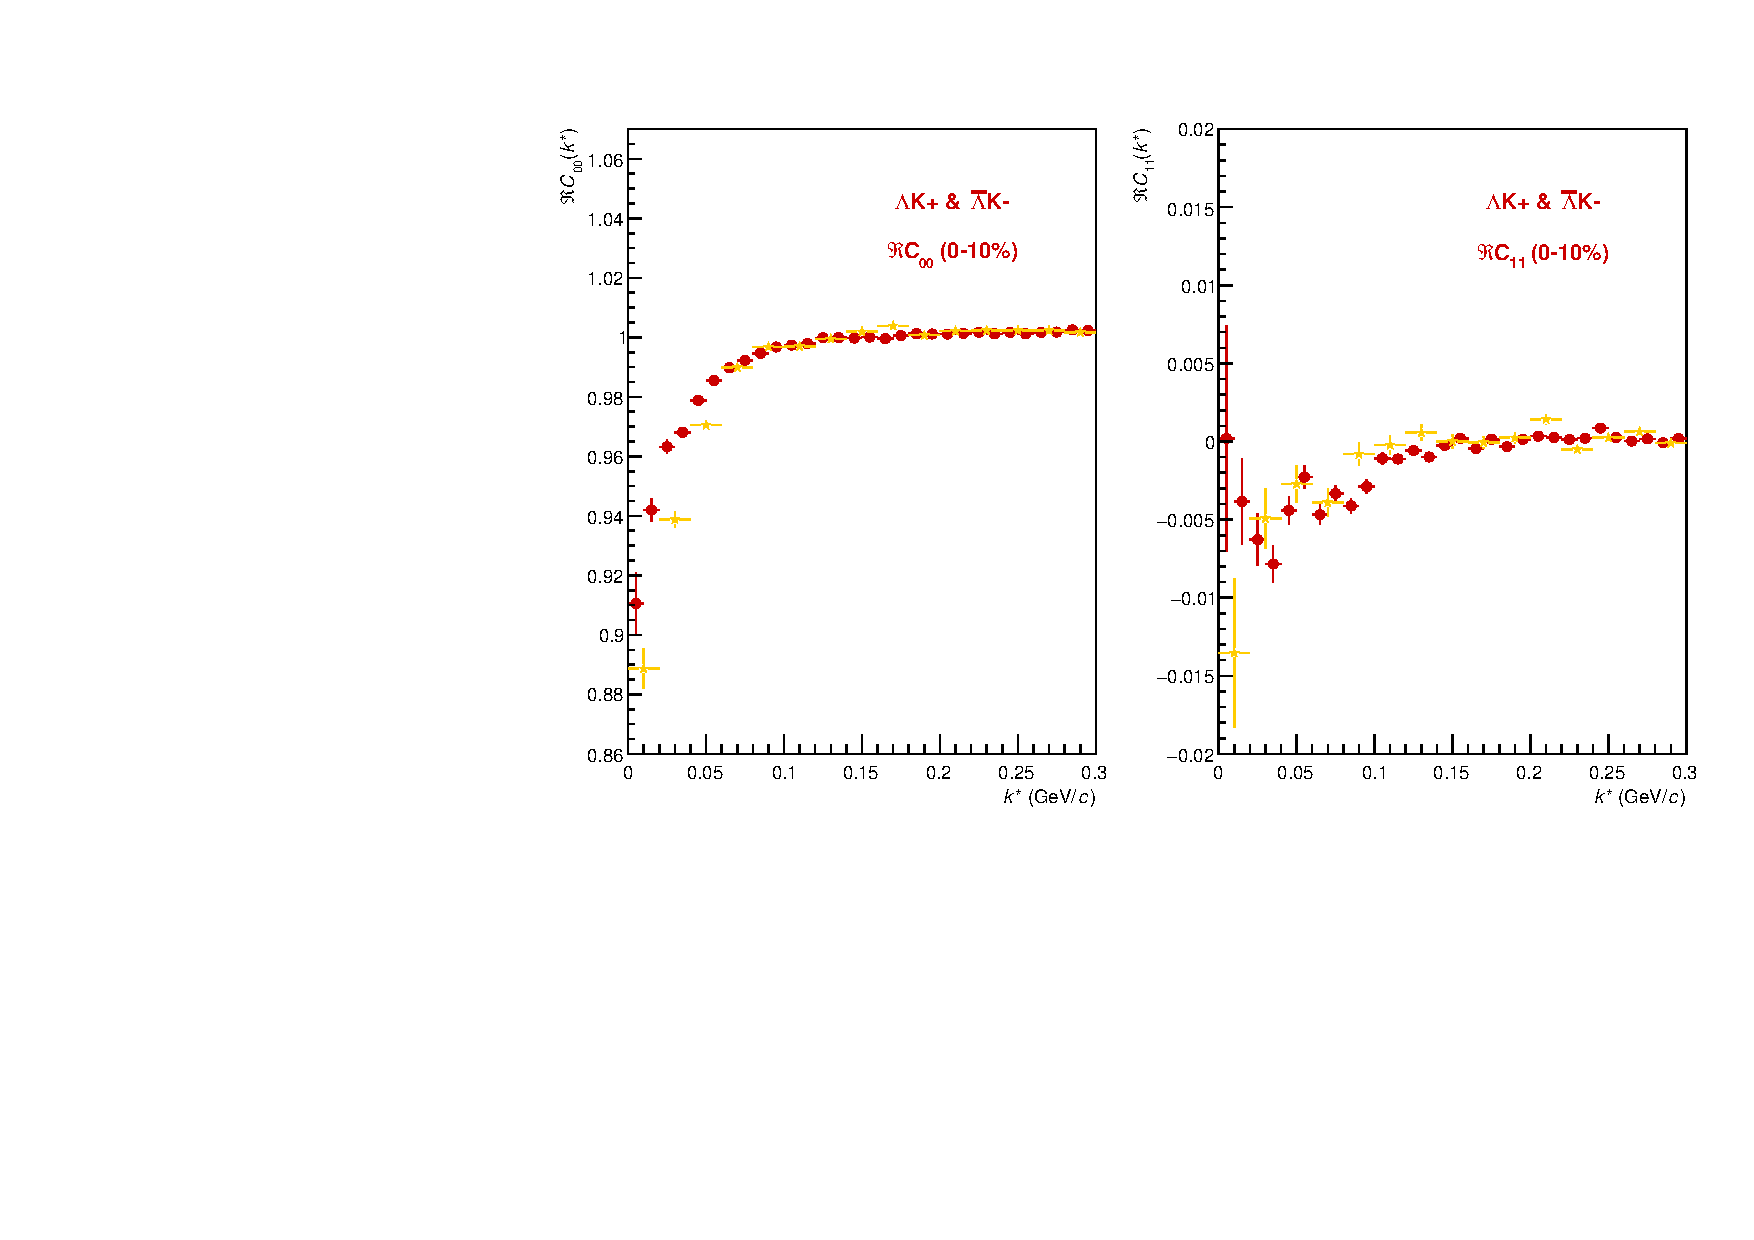
\includegraphics[width=0.8\textwidth]{\ResultsDirBase Results_cLamcKch_20181205/SphericalHarmonics/LamKchP/CanCfYlmReC00C11_LamKchPALamKchM_0010.pdf}
  \caption[\LamKchP $C_{00}$ and $\Re C_{11}$ Spherical Harmonic Components (0-10\%)]{$C_{00}$ (left) and $\Re C_{11}$ (right) components of a spherical harmonic decomposition of the \LamKchP correlation function for the 0-10\% centrality bin.  
The $C_{00}$ component is similar to the 1D correlation functions typically studied, and probes the overall size of the source.
The $\Re C_{11}$ component probes the asymmetry in the system; a non-zero value reveals the asymmetry}
  \label{fig:LamKchP_ReC00C11_0010}
\end{figure}



\section{Relative Emission Shifts with THERMINATOR 2}
\label{app:THERM}

Fig. \ref{fig:LamKchP_StdThermSources} shows results from the THERMINATOR 2 event generator for an impact parameter of b = 2 fm.
As THERMINATOR does not include any final state effects, the femtoscopic correlation was introduced by assuming a set of scattering parameters ($\Re f_{0}, \Im f_{0}, d_{0}$) = (-1.16, 0.51, 1.08) and weighting the signal distribution (numerator pairs) with the modulus squared of the two-particle wave function, $|\Psi|^{2}$.

The top left of Fig. \ref{fig:LamKchP_StdThermSources_Spatial} shows a fit to the one-dimensional correlation function from THERMINATOR 2.
The scattering parameters are known precisely here, as they served as the weights used in the simulation, and are kept constant in the fit.
We are interested in looking at the extracted one-dimensional source size here, so the $\lambda$ parameter is also fixed at unity.
The other three plots in Fig. \ref{fig:LamKchP_StdThermSources_Spatial} show the source distribution in the out (top right), side (bottom left), and long (bottom right) directions (all in the PRF).
The source distributions have all been fitted with a Gaussian form, the result of which is printed within the respective plot.
One immediately sees a significant shift in the out direction, $\mu_{\mathrm{out}} \approx$ 4 fm, and negligible shift in the other two directions, $\mu_{\mathrm{side}} \approx \mu_{\mathrm{long}} \approx$ 0 fm.
The figure demonstrates that, within the THERMINATOR 2 model, the \Lam is, on average, emitted further out that its K partner.
Finally, Fig. \ref{fig:LamKchP_StdThermSources_Temporal} shows the distribution of the relative time of emittance, again in the PRF.
The figure shows that the \Lam is, on average, emitted earlier than its K partner. 

We end this section with a brief look at how a spatial separation of the single particle sources affects the radii extracted from a femtoscopic analysis.
To achieve this, we use THERMINATOR 2 in a similar fashion as described above, but with one important difference.
Instead of taking the source information from THERMINATOR 2, we instead draw the source from a pre-determined Gaussian distribution.
In all cases, we take $R_{\mathrm{out}} = R_{\mathrm{side}} = R_{\mathrm{long}}$ = 5 fm, and $\mu_{\mathrm{side}} = \mu_{\mathrm{long}}$ = 0 fm.
In Figure \ref{fig:LamKchP_ThermSources_VaryMuOut}, we show results for the case of $\mu_{out}$ = 1 fm, $\mu_{out}$ = 3 fm, and $\mu_{out}$ = 6 fm.
In this figure, we do not show the side and long distributions, as they are simple Gaussians of width 5 fm centered about the origin.
The figure demonstrates that as the separation $\mu_{out}$ increases, so do the extracted femtoscopic radii.

\begin{figure}[h!]
  \centering
  %%----start of first subfigure---  
  \subfigure[(Top Left) Simple fit on simulation from THERMINATOR 2. Generated source in the (Top Right) out, (Bottom Left) side, and (Bottom Right) long directions.]{
    \label{fig:LamKchP_StdThermSources_Spatial}
    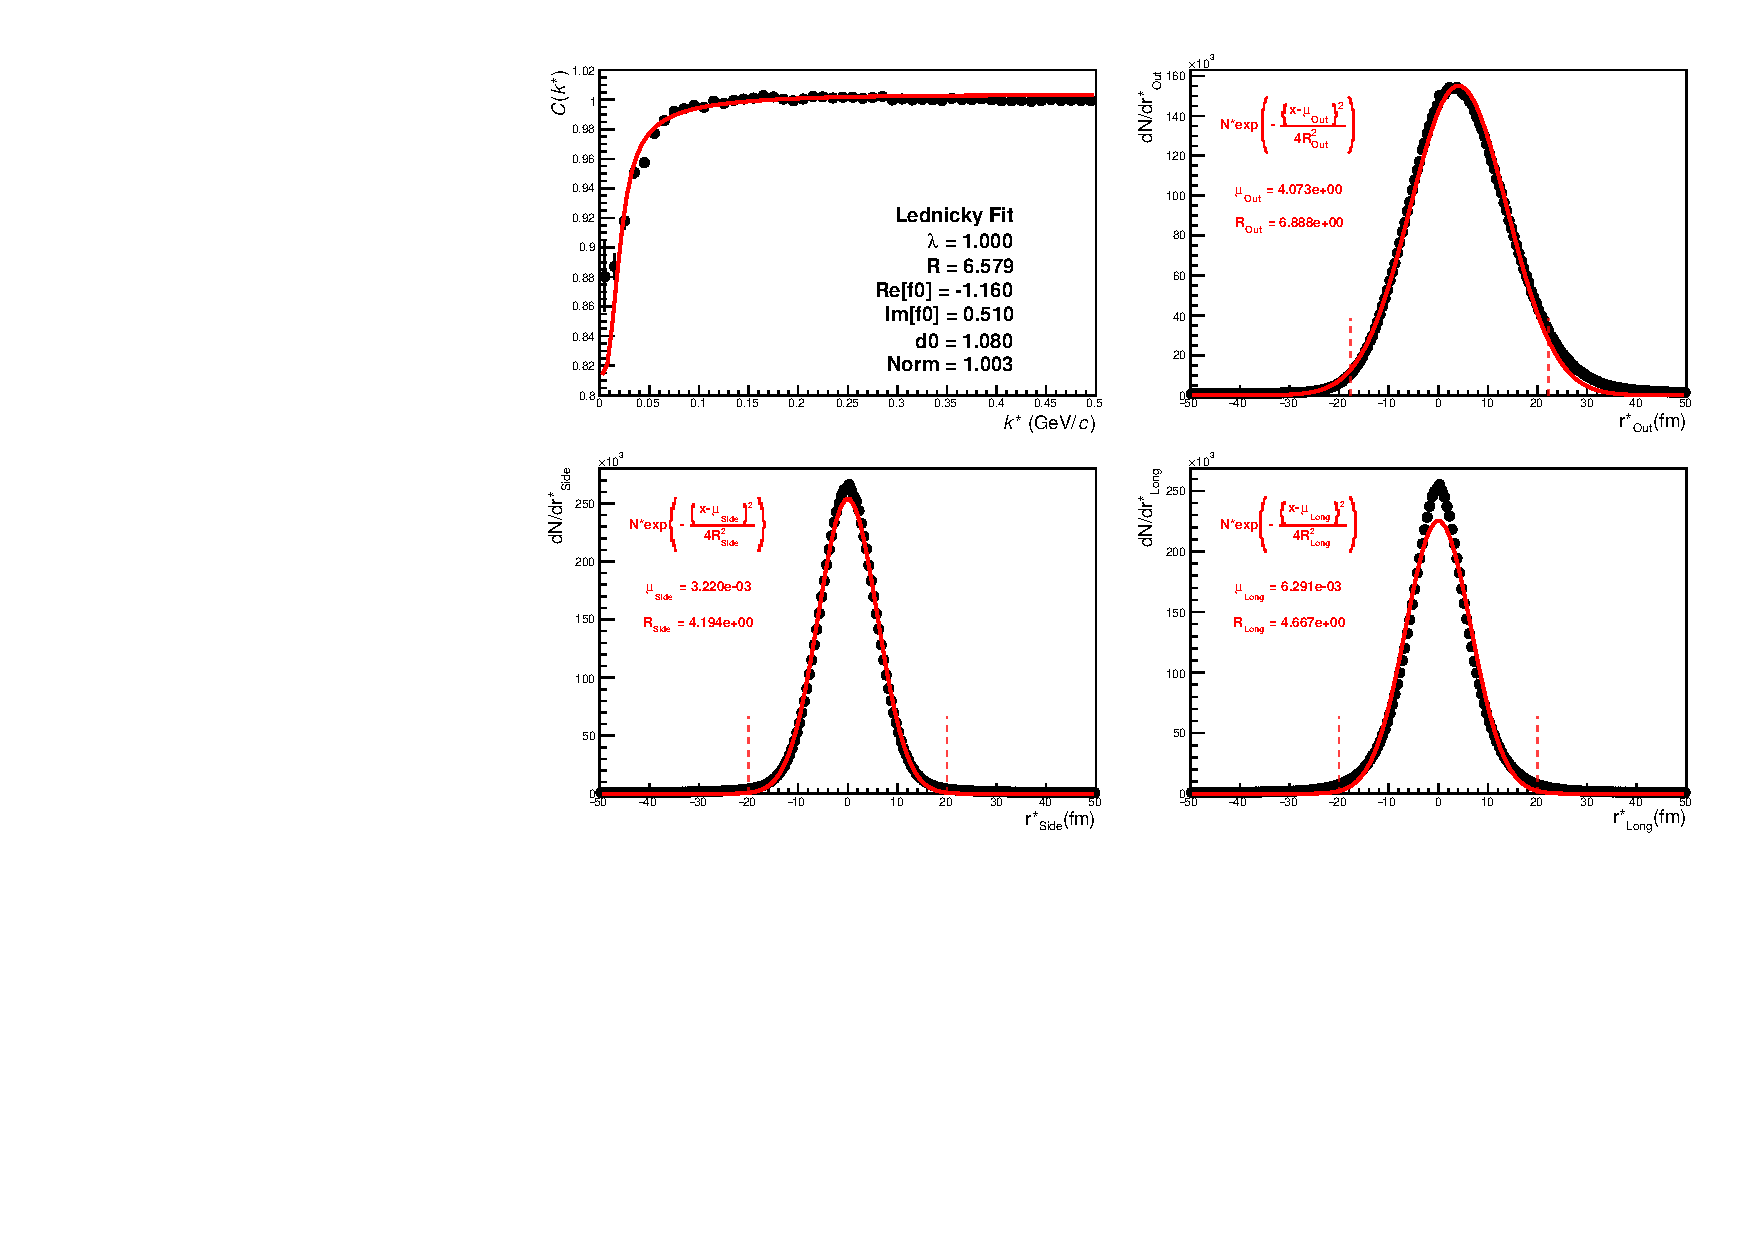
\includegraphics[width=\linewidth]{/home/jesse/Analysis/FemtoAnalysis/AnalysisNotes/7_ResultsAndDiscussion/7.1_ResultsLamK/7.1.5_ResultsLamK_DiscussionOfmTScaling/ThermPlots/LamKchP/CanCfwSource_Full_LamKchP_3dHistPairSource3d_oslLamKchP_FromFileCorrelationFunctions_wOtherPairs.pdf}} \\
  %%----start of second subfigure---
  \subfigure[Temporal characteristics of the source.]{
    \label{fig:LamKchP_StdThermSources_Temporal}
    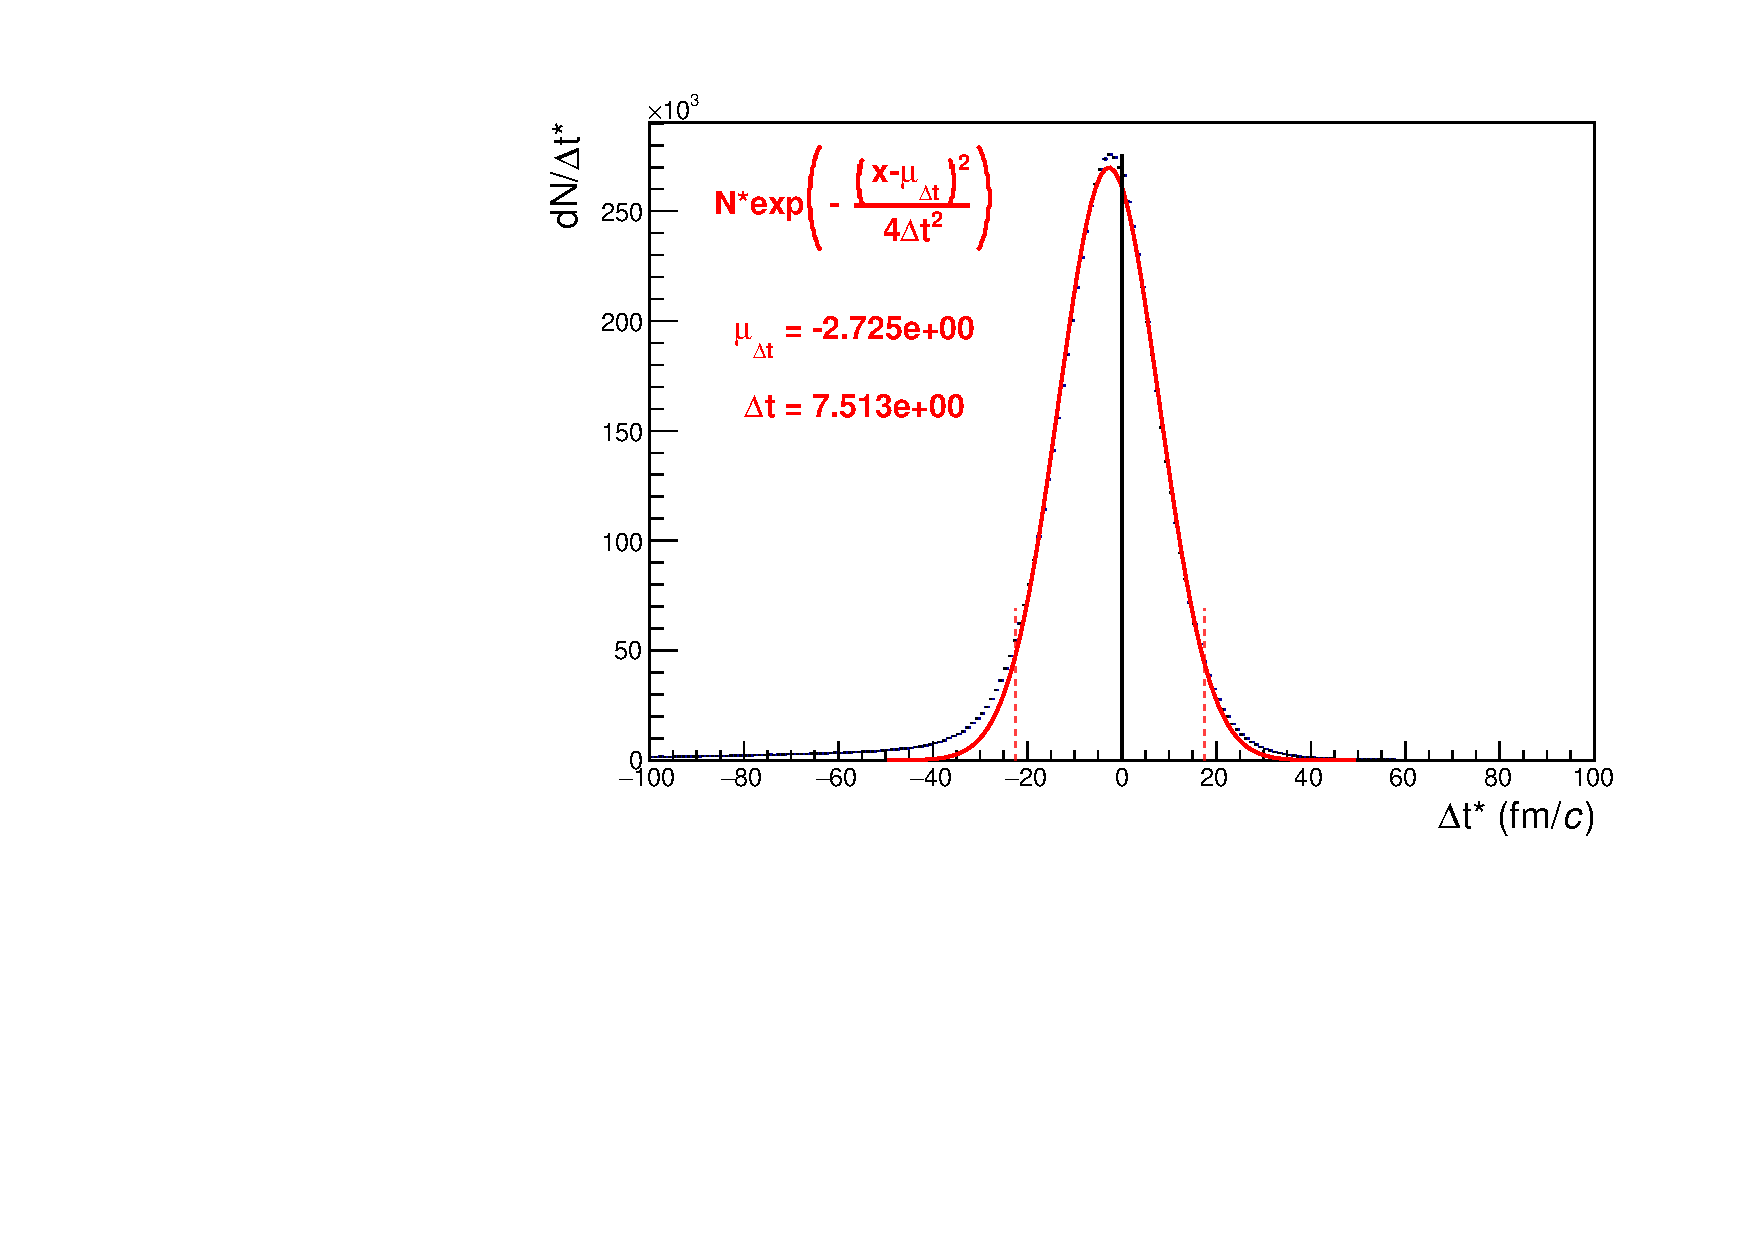
\includegraphics[width=0.60\linewidth]{/home/jesse/Analysis/FemtoAnalysis/AnalysisNotes/7_ResultsAndDiscussion/7.1_ResultsLamK/7.1.5_ResultsLamK_DiscussionOfmTScaling/ThermPlots/LamKchP/CanDeltaT_Full_LamKchP_FromFileCorrelationFunctions_wOtherPairs_BuildCfYlm.pdf}}  
  %%----overall caption----
  \caption[Extracted Radius and Pair Sources from THERMINATOR 2]{Extracted radius when performing a simple fit on simulation from THERMINATOR 2, along with the spatio-temporal characteristics generated by the simulation.}
  \label{fig:LamKchP_StdThermSources}
\end{figure}



\begin{figure}[h]
  \centering
  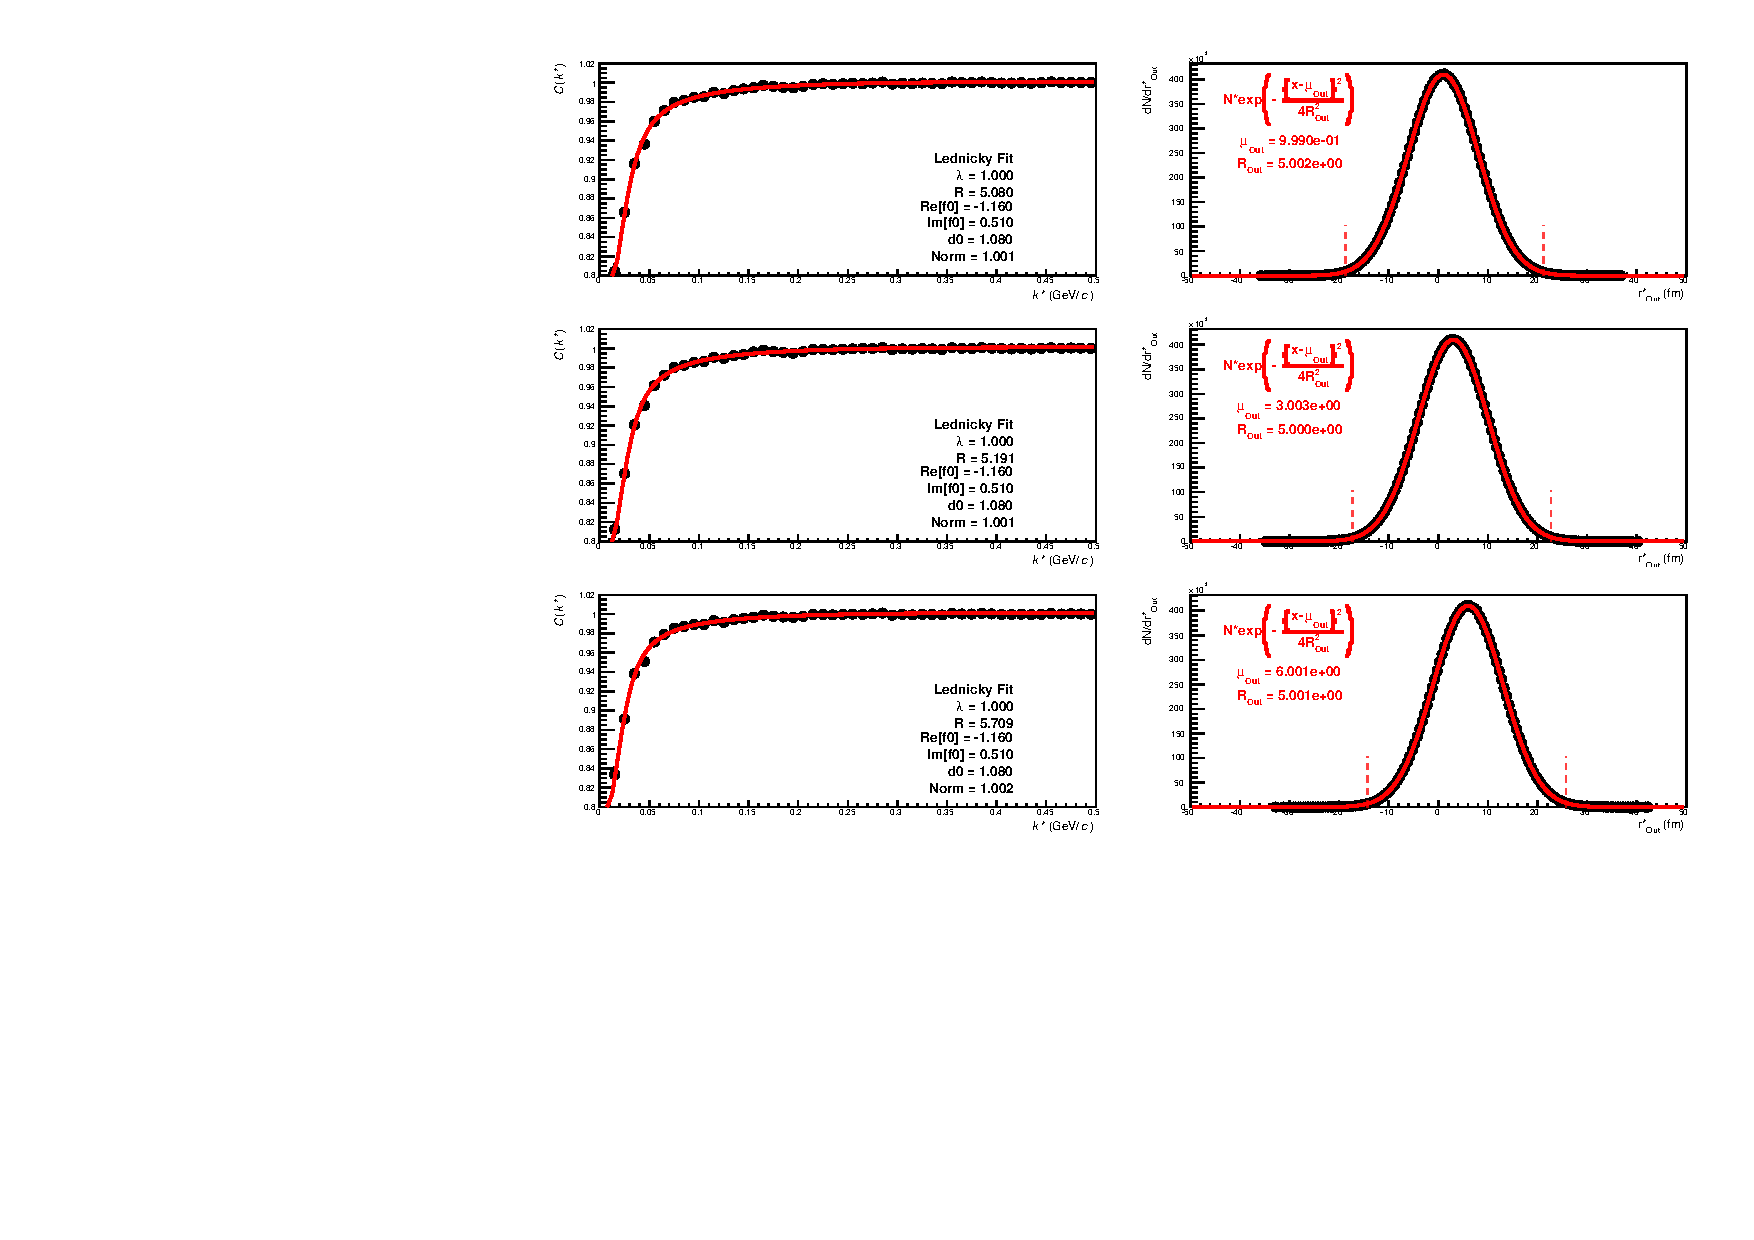
\includegraphics[width=\textwidth]{/home/jesse/Analysis/FemtoAnalysis/AnalysisNotes/7_ResultsAndDiscussion/7.1_ResultsLamK/7.1.5_ResultsLamK_DiscussionOfmTScaling/ThermPlots/LamKchP/CanCompMus_Full_LamKchP_3dHistPairSource3d_oslLamKchP.pdf}
  \caption[Varying $\mu_{\mathrm{Out}}$ with THERMINATOR 2]{Probing the effect of varying the source shift in the outward direction, $\mu_{\mathrm{Out}}$, within the THERMINATOR 2 framework.  To achieve this, we formed particle pairs from the simulation, but altered their spatial characteristics by drawing the out, side, and long components from pre-determined Gaussian distributions.  The plots on the left show fits resulting from the sources (in the out direction) shown on the right.  The sources in the side and long directions are not shown, and are both Gaussians of width 5 fm centered at the origin for all cases.  Moving from top to bottom, $\mu_{\mathrm{Out}}$ increase from 0 to 6 fm, the effect of which clearly increases the effective radius extracted in the fit.}
  \label{fig:LamKchP_ThermSources_VaryMuOut}
\end{figure}

\clearpage



\section{The ALICE Collaboration}
\label{app:collab}
%\input{authorlist-preprint.tex}  %%%%%%% done by webmaster team
\end{document}
